\documentclass[10pt]{article}
\usepackage[preprint]{tmlr}
% preprint option: de-anonymised, no journal header

\usepackage[T1]{fontenc}
\usepackage[utf8]{inputenc}
\usepackage{hyperref}
\usepackage{url}
\usepackage{graphicx}
\usepackage{booktabs}
\usepackage{amsmath,amssymb}
\usepackage{textcomp}
\graphicspath{{figures/}{../../../figures/v3/}}

% generated by scripts/97_paper_numbers_v3.py from results/; do not edit
\makeatletter
\newcommand{\val}[1]{\@ifundefined{val@#1}{\textbf{??#1??}}{\csname val@#1\endcsname}}
\expandafter\def\csname val@af.A.E0_tijepa0.af\endcsname{0.711}
\expandafter\def\csname val@af.A.E0_tijepa0.af.ci\endcsname{0.667--0.748}
\expandafter\def\csname val@af.A.E0_tijepa0.all\endcsname{0.749}
\expandafter\def\csname val@af.A.E0_tijepa0.all.ci\endcsname{0.709--0.783}
\expandafter\def\csname val@af.A.E0_tijepa0.dodt\endcsname{0.682}
\expandafter\def\csname val@af.A.E0_tijepa0.dodt.ci\endcsname{0.637--0.718}
\expandafter\def\csname val@af.A.E1_handcrafted.all\endcsname{0.742}
\expandafter\def\csname val@af.A.E1_handcrafted.all.ci\endcsname{0.699--0.775}
\expandafter\def\csname val@af.A.E2_imagenet_vit_s.af\endcsname{0.690}
\expandafter\def\csname val@af.A.E2_imagenet_vit_s.af.ci\endcsname{0.646--0.730}
\expandafter\def\csname val@af.A.E2_imagenet_vit_s.all\endcsname{0.714}
\expandafter\def\csname val@af.A.E2_imagenet_vit_s.all.ci\endcsname{0.667--0.752}
\expandafter\def\csname val@af.A.E2_imagenet_vit_s.dodt\endcsname{0.668}
\expandafter\def\csname val@af.A.E2_imagenet_vit_s.dodt.ci\endcsname{0.630--0.697}
\expandafter\def\csname val@af.A.E3_dinov2_vit_s.af\endcsname{0.713}
\expandafter\def\csname val@af.A.E3_dinov2_vit_s.af.ci\endcsname{0.669--0.750}
\expandafter\def\csname val@af.A.E3_dinov2_vit_s.all\endcsname{0.730}
\expandafter\def\csname val@af.A.E3_dinov2_vit_s.all.ci\endcsname{0.684--0.770}
\expandafter\def\csname val@af.A.E3_dinov2_vit_s.dodt\endcsname{0.663}
\expandafter\def\csname val@af.A.E3_dinov2_vit_s.dodt.ci\endcsname{0.617--0.700}
\expandafter\def\csname val@af.A.E4_tijepa1.af\endcsname{0.716}
\expandafter\def\csname val@af.A.E4_tijepa1.af.ci\endcsname{0.672--0.748}
\expandafter\def\csname val@af.A.E4_tijepa1.all\endcsname{0.735}
\expandafter\def\csname val@af.A.E4_tijepa1.all.ci\endcsname{0.695--0.768}
\expandafter\def\csname val@af.A.E4_tijepa1.dodt\endcsname{0.671}
\expandafter\def\csname val@af.A.E4_tijepa1.dodt.ci\endcsname{0.623--0.710}
\expandafter\def\csname val@af.A.E4s_tijepa1_spatial.af\endcsname{0.720}
\expandafter\def\csname val@af.A.E4s_tijepa1_spatial.af.ci\endcsname{0.675--0.757}
\expandafter\def\csname val@af.A.E4s_tijepa1_spatial.all\endcsname{0.735}
\expandafter\def\csname val@af.A.E4s_tijepa1_spatial.all.ci\endcsname{0.689--0.770}
\expandafter\def\csname val@af.A.E4s_tijepa1_spatial.dodt\endcsname{0.660}
\expandafter\def\csname val@af.A.E4s_tijepa1_spatial.dodt.ci\endcsname{0.604--0.705}
\expandafter\def\csname val@af.A.E6_random_init_draw0.af\endcsname{0.692}
\expandafter\def\csname val@af.A.E6_random_init_draw0.af.ci\endcsname{0.651--0.726}
\expandafter\def\csname val@af.A.E6_random_init_draw0.all\endcsname{0.722}
\expandafter\def\csname val@af.A.E6_random_init_draw0.all.ci\endcsname{0.680--0.753}
\expandafter\def\csname val@af.A.E6_random_init_draw0.dodt\endcsname{0.634}
\expandafter\def\csname val@af.A.E6_random_init_draw0.dodt.ci\endcsname{0.592--0.667}
\expandafter\def\csname val@af.A.E6_random_init_draw1.af\endcsname{0.693}
\expandafter\def\csname val@af.A.E6_random_init_draw1.af.ci\endcsname{0.651--0.725}
\expandafter\def\csname val@af.A.E6_random_init_draw1.all\endcsname{0.724}
\expandafter\def\csname val@af.A.E6_random_init_draw1.all.ci\endcsname{0.682--0.755}
\expandafter\def\csname val@af.A.E6_random_init_draw1.dodt\endcsname{0.640}
\expandafter\def\csname val@af.A.E6_random_init_draw1.dodt.ci\endcsname{0.593--0.677}
\expandafter\def\csname val@af.A.E6_random_init_draw2.af\endcsname{0.696}
\expandafter\def\csname val@af.A.E6_random_init_draw2.af.ci\endcsname{0.653--0.731}
\expandafter\def\csname val@af.A.E6_random_init_draw2.all\endcsname{0.728}
\expandafter\def\csname val@af.A.E6_random_init_draw2.all.ci\endcsname{0.686--0.758}
\expandafter\def\csname val@af.A.E6_random_init_draw2.dodt\endcsname{0.640}
\expandafter\def\csname val@af.A.E6_random_init_draw2.dodt.ci\endcsname{0.600--0.673}
\expandafter\def\csname val@af.A.E7_vjepa2_vitl.af\endcsname{0.715}
\expandafter\def\csname val@af.A.E7_vjepa2_vitl.af.ci\endcsname{0.668--0.751}
\expandafter\def\csname val@af.A.E7_vjepa2_vitl.all\endcsname{0.753}
\expandafter\def\csname val@af.A.E7_vjepa2_vitl.all.ci\endcsname{0.699--0.790}
\expandafter\def\csname val@af.A.E7_vjepa2_vitl.dodt\endcsname{0.714}
\expandafter\def\csname val@af.A.E7_vjepa2_vitl.dodt.ci\endcsname{0.672--0.747}
\expandafter\def\csname val@af.A.fovs\endcsname{31}
\expandafter\def\csname val@af.A.frozen.max\endcsname{0.753}
\expandafter\def\csname val@af.A.frozen.min\endcsname{0.714}
\expandafter\def\csname val@af.A.intensity_baseline.all\endcsname{0.741}
\expandafter\def\csname val@af.A.intensity_baseline.all.ci\endcsname{0.694--0.775}
\expandafter\def\csname val@af.A.n\endcsname{5{,}078}
\expandafter\def\csname val@af.Am.E0_tijepa0.af\endcsname{0.692}
\expandafter\def\csname val@af.Am.E0_tijepa0.af.ci\endcsname{0.650--0.726}
\expandafter\def\csname val@af.Am.E0_tijepa0.all\endcsname{0.721}
\expandafter\def\csname val@af.Am.E0_tijepa0.all.ci\endcsname{0.680--0.755}
\expandafter\def\csname val@af.Am.E0_tijepa0.dodt\endcsname{0.674}
\expandafter\def\csname val@af.Am.E0_tijepa0.dodt.ci\endcsname{0.630--0.702}
\expandafter\def\csname val@af.Am.E1_handcrafted.all\endcsname{0.710}
\expandafter\def\csname val@af.Am.E1_handcrafted.all.ci\endcsname{0.651--0.744}
\expandafter\def\csname val@af.Am.E2_imagenet_vit_s.af\endcsname{0.660}
\expandafter\def\csname val@af.Am.E2_imagenet_vit_s.af.ci\endcsname{0.632--0.697}
\expandafter\def\csname val@af.Am.E2_imagenet_vit_s.all\endcsname{0.686}
\expandafter\def\csname val@af.Am.E2_imagenet_vit_s.all.ci\endcsname{0.640--0.719}
\expandafter\def\csname val@af.Am.E2_imagenet_vit_s.dodt\endcsname{0.650}
\expandafter\def\csname val@af.Am.E2_imagenet_vit_s.dodt.ci\endcsname{0.600--0.678}
\expandafter\def\csname val@af.Am.E3_dinov2_vit_s.af\endcsname{0.678}
\expandafter\def\csname val@af.Am.E3_dinov2_vit_s.af.ci\endcsname{0.639--0.718}
\expandafter\def\csname val@af.Am.E3_dinov2_vit_s.all\endcsname{0.681}
\expandafter\def\csname val@af.Am.E3_dinov2_vit_s.all.ci\endcsname{0.635--0.714}
\expandafter\def\csname val@af.Am.E3_dinov2_vit_s.dodt\endcsname{0.644}
\expandafter\def\csname val@af.Am.E3_dinov2_vit_s.dodt.ci\endcsname{0.595--0.679}
\expandafter\def\csname val@af.Am.E4_tijepa1.af\endcsname{0.703}
\expandafter\def\csname val@af.Am.E4_tijepa1.af.ci\endcsname{0.664--0.733}
\expandafter\def\csname val@af.Am.E4_tijepa1.all\endcsname{0.714}
\expandafter\def\csname val@af.Am.E4_tijepa1.all.ci\endcsname{0.674--0.744}
\expandafter\def\csname val@af.Am.E4_tijepa1.dodt\endcsname{0.655}
\expandafter\def\csname val@af.Am.E4_tijepa1.dodt.ci\endcsname{0.604--0.697}
\expandafter\def\csname val@af.Am.E4s_tijepa1_spatial.af\endcsname{0.695}
\expandafter\def\csname val@af.Am.E4s_tijepa1_spatial.af.ci\endcsname{0.650--0.726}
\expandafter\def\csname val@af.Am.E4s_tijepa1_spatial.all\endcsname{0.706}
\expandafter\def\csname val@af.Am.E4s_tijepa1_spatial.all.ci\endcsname{0.660--0.737}
\expandafter\def\csname val@af.Am.E4s_tijepa1_spatial.dodt\endcsname{0.645}
\expandafter\def\csname val@af.Am.E4s_tijepa1_spatial.dodt.ci\endcsname{0.581--0.688}
\expandafter\def\csname val@af.Am.E6_random_init_draw0.af\endcsname{0.683}
\expandafter\def\csname val@af.Am.E6_random_init_draw0.af.ci\endcsname{0.647--0.712}
\expandafter\def\csname val@af.Am.E6_random_init_draw0.all\endcsname{0.696}
\expandafter\def\csname val@af.Am.E6_random_init_draw0.all.ci\endcsname{0.644--0.720}
\expandafter\def\csname val@af.Am.E6_random_init_draw0.dodt\endcsname{0.623}
\expandafter\def\csname val@af.Am.E6_random_init_draw0.dodt.ci\endcsname{0.562--0.650}
\expandafter\def\csname val@af.Am.E6_random_init_draw1.af\endcsname{0.678}
\expandafter\def\csname val@af.Am.E6_random_init_draw1.af.ci\endcsname{0.638--0.705}
\expandafter\def\csname val@af.Am.E6_random_init_draw1.all\endcsname{0.699}
\expandafter\def\csname val@af.Am.E6_random_init_draw1.all.ci\endcsname{0.657--0.730}
\expandafter\def\csname val@af.Am.E6_random_init_draw1.dodt\endcsname{0.626}
\expandafter\def\csname val@af.Am.E6_random_init_draw1.dodt.ci\endcsname{0.571--0.667}
\expandafter\def\csname val@af.Am.E6_random_init_draw2.af\endcsname{0.685}
\expandafter\def\csname val@af.Am.E6_random_init_draw2.af.ci\endcsname{0.646--0.714}
\expandafter\def\csname val@af.Am.E6_random_init_draw2.all\endcsname{0.704}
\expandafter\def\csname val@af.Am.E6_random_init_draw2.all.ci\endcsname{0.659--0.735}
\expandafter\def\csname val@af.Am.E6_random_init_draw2.dodt\endcsname{0.629}
\expandafter\def\csname val@af.Am.E6_random_init_draw2.dodt.ci\endcsname{0.583--0.664}
\expandafter\def\csname val@af.Am.E7_vjepa2_vitl.af\endcsname{0.688}
\expandafter\def\csname val@af.Am.E7_vjepa2_vitl.af.ci\endcsname{0.644--0.723}
\expandafter\def\csname val@af.Am.E7_vjepa2_vitl.all\endcsname{0.718}
\expandafter\def\csname val@af.Am.E7_vjepa2_vitl.all.ci\endcsname{0.668--0.765}
\expandafter\def\csname val@af.Am.E7_vjepa2_vitl.dodt\endcsname{0.696}
\expandafter\def\csname val@af.Am.E7_vjepa2_vitl.dodt.ci\endcsname{0.647--0.731}
\expandafter\def\csname val@af.Am.fovs\endcsname{20}
\expandafter\def\csname val@af.Am.frozen.max\endcsname{0.721}
\expandafter\def\csname val@af.Am.frozen.min\endcsname{0.681}
\expandafter\def\csname val@af.Am.intensity_baseline.all\endcsname{0.714}
\expandafter\def\csname val@af.Am.intensity_baseline.all.ci\endcsname{0.663--0.760}
\expandafter\def\csname val@af.Am.n\endcsname{3{,}975}
\expandafter\def\csname val@af.B.E0_tijepa0.af\endcsname{0.567}
\expandafter\def\csname val@af.B.E0_tijepa0.af.ci\endcsname{0.518--0.687}
\expandafter\def\csname val@af.B.E0_tijepa0.all\endcsname{0.643}
\expandafter\def\csname val@af.B.E0_tijepa0.all.ci\endcsname{0.561--0.783}
\expandafter\def\csname val@af.B.E0_tijepa0.dodt\endcsname{0.661}
\expandafter\def\csname val@af.B.E0_tijepa0.dodt.ci\endcsname{0.588--0.737}
\expandafter\def\csname val@af.B.E1_handcrafted.all\endcsname{0.755}
\expandafter\def\csname val@af.B.E1_handcrafted.all.ci\endcsname{0.675--0.812}
\expandafter\def\csname val@af.B.E2_imagenet_vit_s.af\endcsname{0.648}
\expandafter\def\csname val@af.B.E2_imagenet_vit_s.af.ci\endcsname{0.594--0.770}
\expandafter\def\csname val@af.B.E2_imagenet_vit_s.all\endcsname{0.715}
\expandafter\def\csname val@af.B.E2_imagenet_vit_s.all.ci\endcsname{0.653--0.835}
\expandafter\def\csname val@af.B.E2_imagenet_vit_s.dodt\endcsname{0.667}
\expandafter\def\csname val@af.B.E2_imagenet_vit_s.dodt.ci\endcsname{0.605--0.751}
\expandafter\def\csname val@af.B.E3_dinov2_vit_s.af\endcsname{0.654}
\expandafter\def\csname val@af.B.E3_dinov2_vit_s.af.ci\endcsname{0.599--0.803}
\expandafter\def\csname val@af.B.E3_dinov2_vit_s.all\endcsname{0.703}
\expandafter\def\csname val@af.B.E3_dinov2_vit_s.all.ci\endcsname{0.630--0.843}
\expandafter\def\csname val@af.B.E3_dinov2_vit_s.dodt\endcsname{0.710}
\expandafter\def\csname val@af.B.E3_dinov2_vit_s.dodt.ci\endcsname{0.631--0.810}
\expandafter\def\csname val@af.B.E4_tijepa1.af\endcsname{0.609}
\expandafter\def\csname val@af.B.E4_tijepa1.af.ci\endcsname{0.541--0.722}
\expandafter\def\csname val@af.B.E4_tijepa1.all\endcsname{0.650}
\expandafter\def\csname val@af.B.E4_tijepa1.all.ci\endcsname{0.554--0.779}
\expandafter\def\csname val@af.B.E4_tijepa1.dodt\endcsname{0.643}
\expandafter\def\csname val@af.B.E4_tijepa1.dodt.ci\endcsname{0.577--0.722}
\expandafter\def\csname val@af.B.E4s_tijepa1_spatial.af\endcsname{0.592}
\expandafter\def\csname val@af.B.E4s_tijepa1_spatial.af.ci\endcsname{0.539--0.692}
\expandafter\def\csname val@af.B.E4s_tijepa1_spatial.all\endcsname{0.656}
\expandafter\def\csname val@af.B.E4s_tijepa1_spatial.all.ci\endcsname{0.568--0.790}
\expandafter\def\csname val@af.B.E4s_tijepa1_spatial.dodt\endcsname{0.620}
\expandafter\def\csname val@af.B.E4s_tijepa1_spatial.dodt.ci\endcsname{0.555--0.707}
\expandafter\def\csname val@af.B.E6_random_init_draw0.af\endcsname{0.516}
\expandafter\def\csname val@af.B.E6_random_init_draw0.af.ci\endcsname{0.470--0.579}
\expandafter\def\csname val@af.B.E6_random_init_draw0.all\endcsname{0.588}
\expandafter\def\csname val@af.B.E6_random_init_draw0.all.ci\endcsname{0.539--0.661}
\expandafter\def\csname val@af.B.E6_random_init_draw0.dodt\endcsname{0.570}
\expandafter\def\csname val@af.B.E6_random_init_draw0.dodt.ci\endcsname{0.490--0.641}
\expandafter\def\csname val@af.B.E6_random_init_draw1.af\endcsname{0.497}
\expandafter\def\csname val@af.B.E6_random_init_draw1.af.ci\endcsname{0.447--0.569}
\expandafter\def\csname val@af.B.E6_random_init_draw1.all\endcsname{0.586}
\expandafter\def\csname val@af.B.E6_random_init_draw1.all.ci\endcsname{0.533--0.657}
\expandafter\def\csname val@af.B.E6_random_init_draw1.dodt\endcsname{0.552}
\expandafter\def\csname val@af.B.E6_random_init_draw1.dodt.ci\endcsname{0.478--0.629}
\expandafter\def\csname val@af.B.E6_random_init_draw2.af\endcsname{0.492}
\expandafter\def\csname val@af.B.E6_random_init_draw2.af.ci\endcsname{0.449--0.546}
\expandafter\def\csname val@af.B.E6_random_init_draw2.all\endcsname{0.571}
\expandafter\def\csname val@af.B.E6_random_init_draw2.all.ci\endcsname{0.520--0.640}
\expandafter\def\csname val@af.B.E6_random_init_draw2.dodt\endcsname{0.551}
\expandafter\def\csname val@af.B.E6_random_init_draw2.dodt.ci\endcsname{0.481--0.627}
\expandafter\def\csname val@af.B.E7_vjepa2_vitl.af\endcsname{0.661}
\expandafter\def\csname val@af.B.E7_vjepa2_vitl.af.ci\endcsname{0.599--0.768}
\expandafter\def\csname val@af.B.E7_vjepa2_vitl.all\endcsname{0.724}
\expandafter\def\csname val@af.B.E7_vjepa2_vitl.all.ci\endcsname{0.660--0.831}
\expandafter\def\csname val@af.B.E7_vjepa2_vitl.dodt\endcsname{0.676}
\expandafter\def\csname val@af.B.E7_vjepa2_vitl.dodt.ci\endcsname{0.606--0.770}
\expandafter\def\csname val@af.B.fovs\endcsname{85}
\expandafter\def\csname val@af.B.frozen.max\endcsname{0.724}
\expandafter\def\csname val@af.B.frozen.min\endcsname{0.571}
\expandafter\def\csname val@af.B.intensity_baseline.all\endcsname{0.680}
\expandafter\def\csname val@af.B.intensity_baseline.all.ci\endcsname{0.571--0.728}
\expandafter\def\csname val@af.B.n\endcsname{3{,}424}
\expandafter\def\csname val@as.E0_tijepa0.both.1\endcsname{0.883}
\expandafter\def\csname val@as.E0_tijepa0.both.3\endcsname{0.851}
\expandafter\def\csname val@as.E0_tijepa0.both.9\endcsname{0.722}
\expandafter\def\csname val@as.E0_tijepa0.both.idf1\endcsname{0.401}
\expandafter\def\csname val@as.E0_tijepa0.emb.1\endcsname{0.759}
\expandafter\def\csname val@as.E0_tijepa0.emb.3\endcsname{0.668}
\expandafter\def\csname val@as.E0_tijepa0.emb.9\endcsname{0.462}
\expandafter\def\csname val@as.E0_tijepa0.emb.idf1\endcsname{0.224}
\expandafter\def\csname val@as.E0_tijepa0.pos.1\endcsname{0.996}
\expandafter\def\csname val@as.E0_tijepa0.pos.3\endcsname{0.975}
\expandafter\def\csname val@as.E0_tijepa0.pos.9\endcsname{0.876}
\expandafter\def\csname val@as.E0_tijepa0.pos.idf1\endcsname{0.623}
\expandafter\def\csname val@as.E2_imagenet_vit_s.both.1\endcsname{0.986}
\expandafter\def\csname val@as.E2_imagenet_vit_s.both.3\endcsname{0.924}
\expandafter\def\csname val@as.E2_imagenet_vit_s.both.9\endcsname{0.738}
\expandafter\def\csname val@as.E2_imagenet_vit_s.both.idf1\endcsname{0.475}
\expandafter\def\csname val@as.E2_imagenet_vit_s.emb.1\endcsname{0.796}
\expandafter\def\csname val@as.E2_imagenet_vit_s.emb.3\endcsname{0.602}
\expandafter\def\csname val@as.E2_imagenet_vit_s.emb.9\endcsname{0.434}
\expandafter\def\csname val@as.E2_imagenet_vit_s.emb.idf1\endcsname{0.232}
\expandafter\def\csname val@as.E2_imagenet_vit_s.pos.1\endcsname{0.997}
\expandafter\def\csname val@as.E2_imagenet_vit_s.pos.3\endcsname{0.977}
\expandafter\def\csname val@as.E2_imagenet_vit_s.pos.9\endcsname{0.883}
\expandafter\def\csname val@as.E2_imagenet_vit_s.pos.idf1\endcsname{0.625}
\expandafter\def\csname val@as.E3_dinov2_vit_s.both.1\endcsname{0.991}
\expandafter\def\csname val@as.E3_dinov2_vit_s.both.3\endcsname{0.935}
\expandafter\def\csname val@as.E3_dinov2_vit_s.both.9\endcsname{0.771}
\expandafter\def\csname val@as.E3_dinov2_vit_s.both.idf1\endcsname{0.502}
\expandafter\def\csname val@as.E3_dinov2_vit_s.emb.1\endcsname{0.787}
\expandafter\def\csname val@as.E3_dinov2_vit_s.emb.3\endcsname{0.596}
\expandafter\def\csname val@as.E3_dinov2_vit_s.emb.9\endcsname{0.411}
\expandafter\def\csname val@as.E3_dinov2_vit_s.emb.idf1\endcsname{0.208}
\expandafter\def\csname val@as.E3_dinov2_vit_s.pos.1\endcsname{0.997}
\expandafter\def\csname val@as.E3_dinov2_vit_s.pos.3\endcsname{0.977}
\expandafter\def\csname val@as.E3_dinov2_vit_s.pos.9\endcsname{0.883}
\expandafter\def\csname val@as.E3_dinov2_vit_s.pos.idf1\endcsname{0.625}
\expandafter\def\csname val@as.E4_tijepa1.both.1\endcsname{0.857}
\expandafter\def\csname val@as.E4_tijepa1.both.3\endcsname{0.823}
\expandafter\def\csname val@as.E4_tijepa1.both.9\endcsname{0.723}
\expandafter\def\csname val@as.E4_tijepa1.both.idf1\endcsname{0.405}
\expandafter\def\csname val@as.E4_tijepa1.emb.1\endcsname{0.675}
\expandafter\def\csname val@as.E4_tijepa1.emb.3\endcsname{0.587}
\expandafter\def\csname val@as.E4_tijepa1.emb.9\endcsname{0.404}
\expandafter\def\csname val@as.E4_tijepa1.emb.idf1\endcsname{0.186}
\expandafter\def\csname val@as.E4_tijepa1.pos.1\endcsname{0.997}
\expandafter\def\csname val@as.E4_tijepa1.pos.3\endcsname{0.977}
\expandafter\def\csname val@as.E4_tijepa1.pos.9\endcsname{0.883}
\expandafter\def\csname val@as.E4_tijepa1.pos.idf1\endcsname{0.625}
\expandafter\def\csname val@as.E4s_tijepa1_spatial.both.1\endcsname{0.744}
\expandafter\def\csname val@as.E4s_tijepa1_spatial.both.3\endcsname{0.696}
\expandafter\def\csname val@as.E4s_tijepa1_spatial.both.9\endcsname{0.589}
\expandafter\def\csname val@as.E4s_tijepa1_spatial.both.idf1\endcsname{0.275}
\expandafter\def\csname val@as.E4s_tijepa1_spatial.emb.1\endcsname{0.435}
\expandafter\def\csname val@as.E4s_tijepa1_spatial.emb.3\endcsname{0.367}
\expandafter\def\csname val@as.E4s_tijepa1_spatial.emb.9\endcsname{0.253}
\expandafter\def\csname val@as.E4s_tijepa1_spatial.emb.idf1\endcsname{0.120}
\expandafter\def\csname val@as.E4s_tijepa1_spatial.pos.1\endcsname{0.997}
\expandafter\def\csname val@as.E4s_tijepa1_spatial.pos.3\endcsname{0.977}
\expandafter\def\csname val@as.E4s_tijepa1_spatial.pos.9\endcsname{0.883}
\expandafter\def\csname val@as.E4s_tijepa1_spatial.pos.idf1\endcsname{0.625}
\expandafter\def\csname val@as.E5_frame_shuffled.both.1\endcsname{0.841}
\expandafter\def\csname val@as.E5_frame_shuffled.both.3\endcsname{0.801}
\expandafter\def\csname val@as.E5_frame_shuffled.both.9\endcsname{0.682}
\expandafter\def\csname val@as.E5_frame_shuffled.both.idf1\endcsname{0.358}
\expandafter\def\csname val@as.E5_frame_shuffled.emb.1\endcsname{0.567}
\expandafter\def\csname val@as.E5_frame_shuffled.emb.3\endcsname{0.480}
\expandafter\def\csname val@as.E5_frame_shuffled.emb.9\endcsname{0.314}
\expandafter\def\csname val@as.E5_frame_shuffled.emb.idf1\endcsname{0.136}
\expandafter\def\csname val@as.E5_frame_shuffled.pos.1\endcsname{0.997}
\expandafter\def\csname val@as.E5_frame_shuffled.pos.3\endcsname{0.977}
\expandafter\def\csname val@as.E5_frame_shuffled.pos.9\endcsname{0.883}
\expandafter\def\csname val@as.E5_frame_shuffled.pos.idf1\endcsname{0.625}
\expandafter\def\csname val@as.E6_random_init_draw0.both.1\endcsname{0.717}
\expandafter\def\csname val@as.E6_random_init_draw0.both.3\endcsname{0.682}
\expandafter\def\csname val@as.E6_random_init_draw0.both.9\endcsname{0.585}
\expandafter\def\csname val@as.E6_random_init_draw0.both.idf1\endcsname{0.279}
\expandafter\def\csname val@as.E6_random_init_draw0.emb.1\endcsname{0.400}
\expandafter\def\csname val@as.E6_random_init_draw0.emb.3\endcsname{0.330}
\expandafter\def\csname val@as.E6_random_init_draw0.emb.9\endcsname{0.208}
\expandafter\def\csname val@as.E6_random_init_draw0.emb.idf1\endcsname{0.097}
\expandafter\def\csname val@as.E6_random_init_draw0.pos.1\endcsname{0.997}
\expandafter\def\csname val@as.E6_random_init_draw0.pos.3\endcsname{0.977}
\expandafter\def\csname val@as.E6_random_init_draw0.pos.9\endcsname{0.883}
\expandafter\def\csname val@as.E6_random_init_draw0.pos.idf1\endcsname{0.625}
\expandafter\def\csname val@as.E6_random_init_draw1.both.1\endcsname{0.713}
\expandafter\def\csname val@as.E6_random_init_draw1.both.3\endcsname{0.675}
\expandafter\def\csname val@as.E6_random_init_draw1.both.9\endcsname{0.576}
\expandafter\def\csname val@as.E6_random_init_draw1.both.idf1\endcsname{0.267}
\expandafter\def\csname val@as.E6_random_init_draw1.emb.1\endcsname{0.402}
\expandafter\def\csname val@as.E6_random_init_draw1.emb.3\endcsname{0.334}
\expandafter\def\csname val@as.E6_random_init_draw1.emb.9\endcsname{0.214}
\expandafter\def\csname val@as.E6_random_init_draw1.emb.idf1\endcsname{0.098}
\expandafter\def\csname val@as.E6_random_init_draw1.pos.1\endcsname{0.997}
\expandafter\def\csname val@as.E6_random_init_draw1.pos.3\endcsname{0.977}
\expandafter\def\csname val@as.E6_random_init_draw1.pos.9\endcsname{0.883}
\expandafter\def\csname val@as.E6_random_init_draw1.pos.idf1\endcsname{0.625}
\expandafter\def\csname val@as.E6_random_init_draw2.both.1\endcsname{0.716}
\expandafter\def\csname val@as.E6_random_init_draw2.both.3\endcsname{0.679}
\expandafter\def\csname val@as.E6_random_init_draw2.both.9\endcsname{0.583}
\expandafter\def\csname val@as.E6_random_init_draw2.both.idf1\endcsname{0.280}
\expandafter\def\csname val@as.E6_random_init_draw2.emb.1\endcsname{0.416}
\expandafter\def\csname val@as.E6_random_init_draw2.emb.3\endcsname{0.342}
\expandafter\def\csname val@as.E6_random_init_draw2.emb.9\endcsname{0.221}
\expandafter\def\csname val@as.E6_random_init_draw2.emb.idf1\endcsname{0.100}
\expandafter\def\csname val@as.E6_random_init_draw2.pos.1\endcsname{0.997}
\expandafter\def\csname val@as.E6_random_init_draw2.pos.3\endcsname{0.977}
\expandafter\def\csname val@as.E6_random_init_draw2.pos.9\endcsname{0.883}
\expandafter\def\csname val@as.E6_random_init_draw2.pos.idf1\endcsname{0.625}
\expandafter\def\csname val@as.E7_vjepa2_vitl.both.1\endcsname{0.998}
\expandafter\def\csname val@as.E7_vjepa2_vitl.both.3\endcsname{0.986}
\expandafter\def\csname val@as.E7_vjepa2_vitl.both.9\endcsname{0.875}
\expandafter\def\csname val@as.E7_vjepa2_vitl.both.idf1\endcsname{0.624}
\expandafter\def\csname val@as.E7_vjepa2_vitl.emb.1\endcsname{0.994}
\expandafter\def\csname val@as.E7_vjepa2_vitl.emb.3\endcsname{0.967}
\expandafter\def\csname val@as.E7_vjepa2_vitl.emb.9\endcsname{0.751}
\expandafter\def\csname val@as.E7_vjepa2_vitl.emb.idf1\endcsname{0.450}
\expandafter\def\csname val@as.E7_vjepa2_vitl.pos.1\endcsname{0.997}
\expandafter\def\csname val@as.E7_vjepa2_vitl.pos.3\endcsname{0.977}
\expandafter\def\csname val@as.E7_vjepa2_vitl.pos.9\endcsname{0.883}
\expandafter\def\csname val@as.E7_vjepa2_vitl.pos.idf1\endcsname{0.625}
\expandafter\def\csname val@as.d.E0_tijepa0.both9\endcsname{-0.154}
\expandafter\def\csname val@as.d.E2_imagenet_vit_s.both9\endcsname{-0.144}
\expandafter\def\csname val@as.d.E3_dinov2_vit_s.both9\endcsname{-0.111}
\expandafter\def\csname val@as.d.E4_tijepa1.both9\endcsname{-0.160}
\expandafter\def\csname val@as.d.E4s_tijepa1_spatial.both9\endcsname{-0.294}
\expandafter\def\csname val@as.d.E5_frame_shuffled.both9\endcsname{-0.201}
\expandafter\def\csname val@as.d.E6_random_init_draw0.both9\endcsname{-0.298}
\expandafter\def\csname val@as.d.E6_random_init_draw1.both9\endcsname{-0.307}
\expandafter\def\csname val@as.d.E6_random_init_draw2.both9\endcsname{-0.299}
\expandafter\def\csname val@as.d.E7_vjepa2_vitl.both9\endcsname{-0.008}
\expandafter\def\csname val@as.p.E0_tijepa0.both9\endcsname{0.062}
\expandafter\def\csname val@as.p.E0_tijepa0.idf1\endcsname{0.062}
\expandafter\def\csname val@as.p.E2_imagenet_vit_s.both9\endcsname{0.031}
\expandafter\def\csname val@as.p.E2_imagenet_vit_s.idf1\endcsname{0.031}
\expandafter\def\csname val@as.p.E3_dinov2_vit_s.both9\endcsname{0.031}
\expandafter\def\csname val@as.p.E3_dinov2_vit_s.idf1\endcsname{0.031}
\expandafter\def\csname val@as.p.E4_tijepa1.both9\endcsname{0.031}
\expandafter\def\csname val@as.p.E4_tijepa1.idf1\endcsname{0.031}
\expandafter\def\csname val@as.p.E4s_tijepa1_spatial.both9\endcsname{0.031}
\expandafter\def\csname val@as.p.E4s_tijepa1_spatial.idf1\endcsname{0.031}
\expandafter\def\csname val@as.p.E5_frame_shuffled.both9\endcsname{0.031}
\expandafter\def\csname val@as.p.E5_frame_shuffled.idf1\endcsname{0.031}
\expandafter\def\csname val@as.p.E6_random_init_draw0.both9\endcsname{0.031}
\expandafter\def\csname val@as.p.E6_random_init_draw0.idf1\endcsname{0.031}
\expandafter\def\csname val@as.p.E6_random_init_draw1.both9\endcsname{0.031}
\expandafter\def\csname val@as.p.E6_random_init_draw1.idf1\endcsname{0.031}
\expandafter\def\csname val@as.p.E6_random_init_draw2.both9\endcsname{0.031}
\expandafter\def\csname val@as.p.E6_random_init_draw2.idf1\endcsname{0.031}
\expandafter\def\csname val@as.p.E7_vjepa2_vitl.both9\endcsname{0.250}
\expandafter\def\csname val@as.p.E7_vjepa2_vitl.idf1\endcsname{0.938}
\expandafter\def\csname val@as.position_only.pos.1\endcsname{0.997}
\expandafter\def\csname val@as.position_only.pos.3\endcsname{0.977}
\expandafter\def\csname val@as.position_only.pos.9\endcsname{0.883}
\expandafter\def\csname val@as.position_only.pos.idf1\endcsname{0.625}
\expandafter\def\csname val@as.t1vs.E3_dinov2_vit_s\endcsname{-0.007}
\expandafter\def\csname val@as.t1vs.E3_dinov2_vit_s.abs\endcsname{0.007}
\expandafter\def\csname val@as.t1vs.E3_dinov2_vit_s.p\endcsname{0.875}
\expandafter\def\csname val@as.t1vs.E4s_tijepa1_spatial\endcsname{+0.151}
\expandafter\def\csname val@as.t1vs.E4s_tijepa1_spatial.abs\endcsname{0.151}
\expandafter\def\csname val@as.t1vs.E4s_tijepa1_spatial.p\endcsname{0.031}
\expandafter\def\csname val@as.t1vs.E5_frame_shuffled\endcsname{+0.089}
\expandafter\def\csname val@as.t1vs.E5_frame_shuffled.abs\endcsname{0.089}
\expandafter\def\csname val@as.t1vs.E5_frame_shuffled.p\endcsname{0.031}
\expandafter\def\csname val@as.t1vs.E6_random_init_draw0\endcsname{+0.195}
\expandafter\def\csname val@as.t1vs.E6_random_init_draw0.abs\endcsname{0.195}
\expandafter\def\csname val@as.t1vs.E6_random_init_draw0.p\endcsname{0.031}
\expandafter\def\csname val@as.t1vs.E7_vjepa2_vitl\endcsname{-0.347}
\expandafter\def\csname val@as.t1vs.E7_vjepa2_vitl.abs\endcsname{0.347}
\expandafter\def\csname val@as.t1vs.E7_vjepa2_vitl.p\endcsname{0.031}
\expandafter\def\csname val@b4.CpG.exp\endcsname{40.5}
\expandafter\def\csname val@b4.CpG.k\endcsname{37}
\expandafter\def\csname val@b4.CpG.or\endcsname{0.79}
\expandafter\def\csname val@b4.CpG.p\endcsname{0.43}
\expandafter\def\csname val@b4.CpG.uni\endcsname{343}
\expandafter\def\csname val@b4.both.exp\endcsname{24.5}
\expandafter\def\csname val@b4.both.k\endcsname{18}
\expandafter\def\csname val@b4.both.or\endcsname{0.58}
\expandafter\def\csname val@b4.both.p\endcsname{0.09}
\expandafter\def\csname val@b4.both.uni\endcsname{343}
\expandafter\def\csname val@b4.h.blunted\endcsname{196}
\expandafter\def\csname val@b4.h.induced\endcsname{1{,}098}
\expandafter\def\csname val@b4.polyIC.exp\endcsname{33.2}
\expandafter\def\csname val@b4.polyIC.k\endcsname{28}
\expandafter\def\csname val@b4.polyIC.or\endcsname{0.69}
\expandafter\def\csname val@b4.polyIC.p\endcsname{0.19}
\expandafter\def\csname val@b4.polyIC.uni\endcsname{343}
\expandafter\def\csname val@bb.E0_tijepa0.3c\endcsname{0.607}
\expandafter\def\csname val@bb.E0_tijepa0.3c.sd\endcsname{0.005}
\expandafter\def\csname val@bb.E0_tijepa0.3c.wb\endcsname{0.622}
\expandafter\def\csname val@bb.E0_tijepa0.ra\endcsname{0.822}
\expandafter\def\csname val@bb.E1_handcrafted_logreg.3c\endcsname{0.499}
\expandafter\def\csname val@bb.E1_handcrafted_logreg.3c.sd\endcsname{0.005}
\expandafter\def\csname val@bb.E1_handcrafted_logreg.3c.wb\endcsname{0.509}
\expandafter\def\csname val@bb.E1_handcrafted_logreg.ra\endcsname{0.705}
\expandafter\def\csname val@bb.E1_handcrafted_rf.3c\endcsname{0.480}
\expandafter\def\csname val@bb.E1_handcrafted_rf.3c.sd\endcsname{0.002}
\expandafter\def\csname val@bb.E1_handcrafted_rf.3c.wb\endcsname{0.487}
\expandafter\def\csname val@bb.E1_handcrafted_rf.ra\endcsname{0.697}
\expandafter\def\csname val@bb.E2_imagenet_vit_s.3c\endcsname{0.590}
\expandafter\def\csname val@bb.E2_imagenet_vit_s.3c.sd\endcsname{0.001}
\expandafter\def\csname val@bb.E2_imagenet_vit_s.3c.wb\endcsname{0.602}
\expandafter\def\csname val@bb.E2_imagenet_vit_s.ra\endcsname{0.756}
\expandafter\def\csname val@bb.E3_dinov2_vit_s.3c\endcsname{0.610}
\expandafter\def\csname val@bb.E3_dinov2_vit_s.3c.sd\endcsname{0.003}
\expandafter\def\csname val@bb.E3_dinov2_vit_s.3c.wb\endcsname{0.622}
\expandafter\def\csname val@bb.E3_dinov2_vit_s.ra\endcsname{0.775}
\expandafter\def\csname val@bb.E4_tijepa1.3c\endcsname{0.595}
\expandafter\def\csname val@bb.E4_tijepa1.3c.sd\endcsname{0.007}
\expandafter\def\csname val@bb.E4_tijepa1.3c.wb\endcsname{0.609}
\expandafter\def\csname val@bb.E4_tijepa1.ra\endcsname{0.818}
\expandafter\def\csname val@bb.E4s_tijepa1_spatial.3c\endcsname{0.582}
\expandafter\def\csname val@bb.E4s_tijepa1_spatial.3c.sd\endcsname{0.008}
\expandafter\def\csname val@bb.E4s_tijepa1_spatial.3c.wb\endcsname{0.598}
\expandafter\def\csname val@bb.E4s_tijepa1_spatial.ra\endcsname{0.806}
\expandafter\def\csname val@bb.E6_random_init.3c\endcsname{0.554}
\expandafter\def\csname val@bb.E6_random_init.3c.sd\endcsname{0.005}
\expandafter\def\csname val@bb.E6_random_init.3c.wb\endcsname{0.564}
\expandafter\def\csname val@bb.E6_random_init.ra\endcsname{0.779}
\expandafter\def\csname val@bb.E7_vjepa2_vitl.3c\endcsname{0.681}
\expandafter\def\csname val@bb.E7_vjepa2_vitl.3c.sd\endcsname{0.001}
\expandafter\def\csname val@bb.E7_vjepa2_vitl.3c.wb\endcsname{0.696}
\expandafter\def\csname val@bb.E7_vjepa2_vitl.ra\endcsname{0.860}
\expandafter\def\csname val@bb.ci.E0_tijepa0.E1_handcrafted_logreg.3c\endcsname{+0.087--+0.129}
\expandafter\def\csname val@bb.ci.E0_tijepa0.E1_handcrafted_logreg.3c.abs\endcsname{0.087--0.129}
\expandafter\def\csname val@bb.ci.E0_tijepa0.E1_handcrafted_logreg.ra\endcsname{+0.094--+0.138}
\expandafter\def\csname val@bb.ci.E0_tijepa0.E1_handcrafted_logreg.ra.abs\endcsname{0.094--0.138}
\expandafter\def\csname val@bb.ci.E0_tijepa0.E1_handcrafted_rf.3c\endcsname{+0.110--+0.146}
\expandafter\def\csname val@bb.ci.E0_tijepa0.E1_handcrafted_rf.3c.abs\endcsname{0.110--0.146}
\expandafter\def\csname val@bb.ci.E0_tijepa0.E1_handcrafted_rf.ra\endcsname{+0.099--+0.151}
\expandafter\def\csname val@bb.ci.E0_tijepa0.E1_handcrafted_rf.ra.abs\endcsname{0.099--0.151}
\expandafter\def\csname val@bb.ci.E0_tijepa0.E2_imagenet_vit_s.3c\endcsname{-0.001--+0.039}
\expandafter\def\csname val@bb.ci.E0_tijepa0.E2_imagenet_vit_s.ra\endcsname{+0.041--+0.089}
\expandafter\def\csname val@bb.ci.E0_tijepa0.E2_imagenet_vit_s.ra.abs\endcsname{0.041--0.089}
\expandafter\def\csname val@bb.ci.E0_tijepa0.E3_dinov2_vit_s.3c\endcsname{-0.019--+0.017}
\expandafter\def\csname val@bb.ci.E0_tijepa0.E3_dinov2_vit_s.ra\endcsname{+0.027--+0.065}
\expandafter\def\csname val@bb.ci.E0_tijepa0.E3_dinov2_vit_s.ra.abs\endcsname{0.027--0.065}
\expandafter\def\csname val@bb.ci.E0_tijepa0.E4_tijepa1.3c\endcsname{-0.004--+0.027}
\expandafter\def\csname val@bb.ci.E0_tijepa0.E4_tijepa1.ra\endcsname{-0.010--+0.021}
\expandafter\def\csname val@bb.ci.E0_tijepa0.E4s_tijepa1_spatial.3c\endcsname{+0.011--+0.042}
\expandafter\def\csname val@bb.ci.E0_tijepa0.E4s_tijepa1_spatial.3c.abs\endcsname{0.011--0.042}
\expandafter\def\csname val@bb.ci.E0_tijepa0.E4s_tijepa1_spatial.ra\endcsname{+0.005--+0.031}
\expandafter\def\csname val@bb.ci.E0_tijepa0.E4s_tijepa1_spatial.ra.abs\endcsname{0.005--0.031}
\expandafter\def\csname val@bb.ci.E0_tijepa0.E6_random_init.3c\endcsname{+0.038--+0.069}
\expandafter\def\csname val@bb.ci.E0_tijepa0.E6_random_init.3c.abs\endcsname{0.038--0.069}
\expandafter\def\csname val@bb.ci.E0_tijepa0.E6_random_init.ra\endcsname{+0.021--+0.063}
\expandafter\def\csname val@bb.ci.E0_tijepa0.E6_random_init.ra.abs\endcsname{0.021--0.063}
\expandafter\def\csname val@bb.ci.E0_tijepa0.E7_vjepa2_vitl.3c\endcsname{-0.091---0.055}
\expandafter\def\csname val@bb.ci.E0_tijepa0.E7_vjepa2_vitl.3c.abs\endcsname{0.055--0.091}
\expandafter\def\csname val@bb.ci.E0_tijepa0.E7_vjepa2_vitl.ra\endcsname{-0.057---0.021}
\expandafter\def\csname val@bb.ci.E0_tijepa0.E7_vjepa2_vitl.ra.abs\endcsname{0.021--0.057}
\expandafter\def\csname val@bb.ci.E1_handcrafted_logreg.E1_handcrafted_rf.3c\endcsname{+0.005--+0.034}
\expandafter\def\csname val@bb.ci.E1_handcrafted_logreg.E1_handcrafted_rf.3c.abs\endcsname{0.005--0.034}
\expandafter\def\csname val@bb.ci.E1_handcrafted_logreg.E1_handcrafted_rf.ra\endcsname{-0.007--+0.022}
\expandafter\def\csname val@bb.ci.E1_handcrafted_logreg.E2_imagenet_vit_s.3c\endcsname{-0.109---0.074}
\expandafter\def\csname val@bb.ci.E1_handcrafted_logreg.E2_imagenet_vit_s.3c.abs\endcsname{0.074--0.109}
\expandafter\def\csname val@bb.ci.E1_handcrafted_logreg.E2_imagenet_vit_s.ra\endcsname{-0.066---0.036}
\expandafter\def\csname val@bb.ci.E1_handcrafted_logreg.E2_imagenet_vit_s.ra.abs\endcsname{0.036--0.066}
\expandafter\def\csname val@bb.ci.E1_handcrafted_logreg.E3_dinov2_vit_s.3c\endcsname{-0.127---0.095}
\expandafter\def\csname val@bb.ci.E1_handcrafted_logreg.E3_dinov2_vit_s.3c.abs\endcsname{0.095--0.127}
\expandafter\def\csname val@bb.ci.E1_handcrafted_logreg.E3_dinov2_vit_s.ra\endcsname{-0.091---0.054}
\expandafter\def\csname val@bb.ci.E1_handcrafted_logreg.E3_dinov2_vit_s.ra.abs\endcsname{0.054--0.091}
\expandafter\def\csname val@bb.ci.E1_handcrafted_logreg.E4_tijepa1.3c\endcsname{-0.115---0.077}
\expandafter\def\csname val@bb.ci.E1_handcrafted_logreg.E4_tijepa1.3c.abs\endcsname{0.077--0.115}
\expandafter\def\csname val@bb.ci.E1_handcrafted_logreg.E4_tijepa1.ra\endcsname{-0.137---0.091}
\expandafter\def\csname val@bb.ci.E1_handcrafted_logreg.E4_tijepa1.ra.abs\endcsname{0.091--0.137}
\expandafter\def\csname val@bb.ci.E1_handcrafted_logreg.E4s_tijepa1_spatial.3c\endcsname{-0.102---0.066}
\expandafter\def\csname val@bb.ci.E1_handcrafted_logreg.E4s_tijepa1_spatial.3c.abs\endcsname{0.066--0.102}
\expandafter\def\csname val@bb.ci.E1_handcrafted_logreg.E4s_tijepa1_spatial.ra\endcsname{-0.124---0.076}
\expandafter\def\csname val@bb.ci.E1_handcrafted_logreg.E4s_tijepa1_spatial.ra.abs\endcsname{0.076--0.124}
\expandafter\def\csname val@bb.ci.E1_handcrafted_logreg.E6_random_init.3c\endcsname{-0.071---0.038}
\expandafter\def\csname val@bb.ci.E1_handcrafted_logreg.E6_random_init.3c.abs\endcsname{0.038--0.071}
\expandafter\def\csname val@bb.ci.E1_handcrafted_logreg.E6_random_init.ra\endcsname{-0.097---0.048}
\expandafter\def\csname val@bb.ci.E1_handcrafted_logreg.E6_random_init.ra.abs\endcsname{0.048--0.097}
\expandafter\def\csname val@bb.ci.E1_handcrafted_logreg.E7_vjepa2_vitl.3c\endcsname{-0.199---0.163}
\expandafter\def\csname val@bb.ci.E1_handcrafted_logreg.E7_vjepa2_vitl.3c.abs\endcsname{0.163--0.199}
\expandafter\def\csname val@bb.ci.E1_handcrafted_logreg.E7_vjepa2_vitl.ra\endcsname{-0.175---0.131}
\expandafter\def\csname val@bb.ci.E1_handcrafted_logreg.E7_vjepa2_vitl.ra.abs\endcsname{0.131--0.175}
\expandafter\def\csname val@bb.ci.E1_handcrafted_rf.E2_imagenet_vit_s.3c\endcsname{-0.127---0.095}
\expandafter\def\csname val@bb.ci.E1_handcrafted_rf.E2_imagenet_vit_s.3c.abs\endcsname{0.095--0.127}
\expandafter\def\csname val@bb.ci.E1_handcrafted_rf.E2_imagenet_vit_s.ra\endcsname{-0.077---0.039}
\expandafter\def\csname val@bb.ci.E1_handcrafted_rf.E2_imagenet_vit_s.ra.abs\endcsname{0.039--0.077}
\expandafter\def\csname val@bb.ci.E1_handcrafted_rf.E3_dinov2_vit_s.3c\endcsname{-0.143---0.114}
\expandafter\def\csname val@bb.ci.E1_handcrafted_rf.E3_dinov2_vit_s.3c.abs\endcsname{0.114--0.143}
\expandafter\def\csname val@bb.ci.E1_handcrafted_rf.E3_dinov2_vit_s.ra\endcsname{-0.102---0.058}
\expandafter\def\csname val@bb.ci.E1_handcrafted_rf.E3_dinov2_vit_s.ra.abs\endcsname{0.058--0.102}
\expandafter\def\csname val@bb.ci.E1_handcrafted_rf.E4_tijepa1.3c\endcsname{-0.132---0.097}
\expandafter\def\csname val@bb.ci.E1_handcrafted_rf.E4_tijepa1.3c.abs\endcsname{0.097--0.132}
\expandafter\def\csname val@bb.ci.E1_handcrafted_rf.E4_tijepa1.ra\endcsname{-0.149---0.097}
\expandafter\def\csname val@bb.ci.E1_handcrafted_rf.E4_tijepa1.ra.abs\endcsname{0.097--0.149}
\expandafter\def\csname val@bb.ci.E1_handcrafted_rf.E4s_tijepa1_spatial.3c\endcsname{-0.119---0.084}
\expandafter\def\csname val@bb.ci.E1_handcrafted_rf.E4s_tijepa1_spatial.3c.abs\endcsname{0.084--0.119}
\expandafter\def\csname val@bb.ci.E1_handcrafted_rf.E4s_tijepa1_spatial.ra\endcsname{-0.137---0.081}
\expandafter\def\csname val@bb.ci.E1_handcrafted_rf.E4s_tijepa1_spatial.ra.abs\endcsname{0.081--0.137}
\expandafter\def\csname val@bb.ci.E1_handcrafted_rf.E6_random_init.3c\endcsname{-0.088---0.056}
\expandafter\def\csname val@bb.ci.E1_handcrafted_rf.E6_random_init.3c.abs\endcsname{0.056--0.088}
\expandafter\def\csname val@bb.ci.E1_handcrafted_rf.E6_random_init.ra\endcsname{-0.104---0.053}
\expandafter\def\csname val@bb.ci.E1_handcrafted_rf.E6_random_init.ra.abs\endcsname{0.053--0.104}
\expandafter\def\csname val@bb.ci.E1_handcrafted_rf.E7_vjepa2_vitl.3c\endcsname{-0.217---0.185}
\expandafter\def\csname val@bb.ci.E1_handcrafted_rf.E7_vjepa2_vitl.3c.abs\endcsname{0.185--0.217}
\expandafter\def\csname val@bb.ci.E1_handcrafted_rf.E7_vjepa2_vitl.ra\endcsname{-0.187---0.136}
\expandafter\def\csname val@bb.ci.E1_handcrafted_rf.E7_vjepa2_vitl.ra.abs\endcsname{0.136--0.187}
\expandafter\def\csname val@bb.ci.E2_imagenet_vit_s.E3_dinov2_vit_s.3c\endcsname{-0.031---0.005}
\expandafter\def\csname val@bb.ci.E2_imagenet_vit_s.E3_dinov2_vit_s.3c.abs\endcsname{0.005--0.031}
\expandafter\def\csname val@bb.ci.E2_imagenet_vit_s.E3_dinov2_vit_s.ra\endcsname{-0.035---0.007}
\expandafter\def\csname val@bb.ci.E2_imagenet_vit_s.E3_dinov2_vit_s.ra.abs\endcsname{0.007--0.035}
\expandafter\def\csname val@bb.ci.E2_imagenet_vit_s.E4_tijepa1.3c\endcsname{-0.024--+0.018}
\expandafter\def\csname val@bb.ci.E2_imagenet_vit_s.E4_tijepa1.ra\endcsname{-0.088---0.040}
\expandafter\def\csname val@bb.ci.E2_imagenet_vit_s.E4_tijepa1.ra.abs\endcsname{0.040--0.088}
\expandafter\def\csname val@bb.ci.E2_imagenet_vit_s.E4s_tijepa1_spatial.3c\endcsname{-0.011--+0.030}
\expandafter\def\csname val@bb.ci.E2_imagenet_vit_s.E4s_tijepa1_spatial.ra\endcsname{-0.074---0.024}
\expandafter\def\csname val@bb.ci.E2_imagenet_vit_s.E4s_tijepa1_spatial.ra.abs\endcsname{0.024--0.074}
\expandafter\def\csname val@bb.ci.E2_imagenet_vit_s.E6_random_init.3c\endcsname{+0.020--+0.057}
\expandafter\def\csname val@bb.ci.E2_imagenet_vit_s.E6_random_init.3c.abs\endcsname{0.020--0.057}
\expandafter\def\csname val@bb.ci.E2_imagenet_vit_s.E6_random_init.ra\endcsname{-0.045--+0.003}
\expandafter\def\csname val@bb.ci.E2_imagenet_vit_s.E7_vjepa2_vitl.3c\endcsname{-0.104---0.077}
\expandafter\def\csname val@bb.ci.E2_imagenet_vit_s.E7_vjepa2_vitl.3c.abs\endcsname{0.077--0.104}
\expandafter\def\csname val@bb.ci.E2_imagenet_vit_s.E7_vjepa2_vitl.ra\endcsname{-0.125---0.079}
\expandafter\def\csname val@bb.ci.E2_imagenet_vit_s.E7_vjepa2_vitl.ra.abs\endcsname{0.079--0.125}
\expandafter\def\csname val@bb.ci.E3_dinov2_vit_s.E4_tijepa1.3c\endcsname{-0.003--+0.033}
\expandafter\def\csname val@bb.ci.E3_dinov2_vit_s.E4_tijepa1.ra\endcsname{-0.063---0.025}
\expandafter\def\csname val@bb.ci.E3_dinov2_vit_s.E4_tijepa1.ra.abs\endcsname{0.025--0.063}
\expandafter\def\csname val@bb.ci.E3_dinov2_vit_s.E4s_tijepa1_spatial.3c\endcsname{+0.011--+0.047}
\expandafter\def\csname val@bb.ci.E3_dinov2_vit_s.E4s_tijepa1_spatial.3c.abs\endcsname{0.011--0.047}
\expandafter\def\csname val@bb.ci.E3_dinov2_vit_s.E4s_tijepa1_spatial.ra\endcsname{-0.050---0.009}
\expandafter\def\csname val@bb.ci.E3_dinov2_vit_s.E4s_tijepa1_spatial.ra.abs\endcsname{0.009--0.050}
\expandafter\def\csname val@bb.ci.E3_dinov2_vit_s.E6_random_init.3c\endcsname{+0.041--+0.074}
\expandafter\def\csname val@bb.ci.E3_dinov2_vit_s.E6_random_init.3c.abs\endcsname{0.041--0.074}
\expandafter\def\csname val@bb.ci.E3_dinov2_vit_s.E6_random_init.ra\endcsname{-0.024--+0.018}
\expandafter\def\csname val@bb.ci.E3_dinov2_vit_s.E7_vjepa2_vitl.3c\endcsname{-0.088---0.057}
\expandafter\def\csname val@bb.ci.E3_dinov2_vit_s.E7_vjepa2_vitl.3c.abs\endcsname{0.057--0.088}
\expandafter\def\csname val@bb.ci.E3_dinov2_vit_s.E7_vjepa2_vitl.ra\endcsname{-0.107---0.065}
\expandafter\def\csname val@bb.ci.E3_dinov2_vit_s.E7_vjepa2_vitl.ra.abs\endcsname{0.065--0.107}
\expandafter\def\csname val@bb.ci.E4_tijepa1.E4s_tijepa1_spatial.3c\endcsname{+0.001--+0.027}
\expandafter\def\csname val@bb.ci.E4_tijepa1.E4s_tijepa1_spatial.3c.abs\endcsname{0.001--0.027}
\expandafter\def\csname val@bb.ci.E4_tijepa1.E4s_tijepa1_spatial.ra\endcsname{-0.004--+0.029}
\expandafter\def\csname val@bb.ci.E4_tijepa1.E6_random_init.3c\endcsname{+0.027--+0.055}
\expandafter\def\csname val@bb.ci.E4_tijepa1.E6_random_init.3c.abs\endcsname{0.027--0.055}
\expandafter\def\csname val@bb.ci.E4_tijepa1.E6_random_init.ra\endcsname{+0.019--+0.059}
\expandafter\def\csname val@bb.ci.E4_tijepa1.E6_random_init.ra.abs\endcsname{0.019--0.059}
\expandafter\def\csname val@bb.ci.E4_tijepa1.E7_vjepa2_vitl.3c\endcsname{-0.108---0.067}
\expandafter\def\csname val@bb.ci.E4_tijepa1.E7_vjepa2_vitl.3c.abs\endcsname{0.067--0.108}
\expandafter\def\csname val@bb.ci.E4_tijepa1.E7_vjepa2_vitl.ra\endcsname{-0.068---0.024}
\expandafter\def\csname val@bb.ci.E4_tijepa1.E7_vjepa2_vitl.ra.abs\endcsname{0.024--0.068}
\expandafter\def\csname val@bb.ci.E4s_tijepa1_spatial.E6_random_init.3c\endcsname{+0.011--+0.041}
\expandafter\def\csname val@bb.ci.E4s_tijepa1_spatial.E6_random_init.3c.abs\endcsname{0.011--0.041}
\expandafter\def\csname val@bb.ci.E4s_tijepa1_spatial.E6_random_init.ra\endcsname{+0.001--+0.049}
\expandafter\def\csname val@bb.ci.E4s_tijepa1_spatial.E6_random_init.ra.abs\endcsname{0.001--0.049}
\expandafter\def\csname val@bb.ci.E4s_tijepa1_spatial.E7_vjepa2_vitl.3c\endcsname{-0.121---0.081}
\expandafter\def\csname val@bb.ci.E4s_tijepa1_spatial.E7_vjepa2_vitl.3c.abs\endcsname{0.081--0.121}
\expandafter\def\csname val@bb.ci.E4s_tijepa1_spatial.E7_vjepa2_vitl.ra\endcsname{-0.072---0.039}
\expandafter\def\csname val@bb.ci.E4s_tijepa1_spatial.E7_vjepa2_vitl.ra.abs\endcsname{0.039--0.072}
\expandafter\def\csname val@bb.ci.E6_random_init.E7_vjepa2_vitl.3c\endcsname{-0.148---0.110}
\expandafter\def\csname val@bb.ci.E6_random_init.E7_vjepa2_vitl.3c.abs\endcsname{0.110--0.148}
\expandafter\def\csname val@bb.ci.E6_random_init.E7_vjepa2_vitl.ra\endcsname{-0.111---0.053}
\expandafter\def\csname val@bb.ci.E6_random_init.E7_vjepa2_vitl.ra.abs\endcsname{0.053--0.111}
\expandafter\def\csname val@bb.d.E0_tijepa0.E1_handcrafted_logreg.3c\endcsname{+0.109}
\expandafter\def\csname val@bb.d.E0_tijepa0.E1_handcrafted_logreg.3c.abs\endcsname{0.109}
\expandafter\def\csname val@bb.d.E0_tijepa0.E1_handcrafted_logreg.ra\endcsname{+0.117}
\expandafter\def\csname val@bb.d.E0_tijepa0.E1_handcrafted_logreg.ra.abs\endcsname{0.117}
\expandafter\def\csname val@bb.d.E0_tijepa0.E1_handcrafted_rf.3c\endcsname{+0.127}
\expandafter\def\csname val@bb.d.E0_tijepa0.E1_handcrafted_rf.3c.abs\endcsname{0.127}
\expandafter\def\csname val@bb.d.E0_tijepa0.E1_handcrafted_rf.ra\endcsname{+0.125}
\expandafter\def\csname val@bb.d.E0_tijepa0.E1_handcrafted_rf.ra.abs\endcsname{0.125}
\expandafter\def\csname val@bb.d.E0_tijepa0.E2_imagenet_vit_s.3c\endcsname{+0.017}
\expandafter\def\csname val@bb.d.E0_tijepa0.E2_imagenet_vit_s.3c.abs\endcsname{0.017}
\expandafter\def\csname val@bb.d.E0_tijepa0.E2_imagenet_vit_s.ra\endcsname{+0.067}
\expandafter\def\csname val@bb.d.E0_tijepa0.E2_imagenet_vit_s.ra.abs\endcsname{0.067}
\expandafter\def\csname val@bb.d.E0_tijepa0.E3_dinov2_vit_s.3c\endcsname{-0.002}
\expandafter\def\csname val@bb.d.E0_tijepa0.E3_dinov2_vit_s.3c.abs\endcsname{0.002}
\expandafter\def\csname val@bb.d.E0_tijepa0.E3_dinov2_vit_s.ra\endcsname{+0.047}
\expandafter\def\csname val@bb.d.E0_tijepa0.E3_dinov2_vit_s.ra.abs\endcsname{0.047}
\expandafter\def\csname val@bb.d.E0_tijepa0.E4_tijepa1.3c\endcsname{+0.012}
\expandafter\def\csname val@bb.d.E0_tijepa0.E4_tijepa1.3c.abs\endcsname{0.012}
\expandafter\def\csname val@bb.d.E0_tijepa0.E4_tijepa1.ra\endcsname{+0.005}
\expandafter\def\csname val@bb.d.E0_tijepa0.E4_tijepa1.ra.abs\endcsname{0.005}
\expandafter\def\csname val@bb.d.E0_tijepa0.E4s_tijepa1_spatial.3c\endcsname{+0.025}
\expandafter\def\csname val@bb.d.E0_tijepa0.E4s_tijepa1_spatial.3c.abs\endcsname{0.025}
\expandafter\def\csname val@bb.d.E0_tijepa0.E4s_tijepa1_spatial.ra\endcsname{+0.017}
\expandafter\def\csname val@bb.d.E0_tijepa0.E4s_tijepa1_spatial.ra.abs\endcsname{0.017}
\expandafter\def\csname val@bb.d.E0_tijepa0.E6_random_init.3c\endcsname{+0.053}
\expandafter\def\csname val@bb.d.E0_tijepa0.E6_random_init.3c.abs\endcsname{0.053}
\expandafter\def\csname val@bb.d.E0_tijepa0.E6_random_init.ra\endcsname{+0.044}
\expandafter\def\csname val@bb.d.E0_tijepa0.E6_random_init.ra.abs\endcsname{0.044}
\expandafter\def\csname val@bb.d.E0_tijepa0.E7_vjepa2_vitl.3c\endcsname{-0.074}
\expandafter\def\csname val@bb.d.E0_tijepa0.E7_vjepa2_vitl.3c.abs\endcsname{0.074}
\expandafter\def\csname val@bb.d.E0_tijepa0.E7_vjepa2_vitl.ra\endcsname{-0.038}
\expandafter\def\csname val@bb.d.E0_tijepa0.E7_vjepa2_vitl.ra.abs\endcsname{0.038}
\expandafter\def\csname val@bb.d.E1_handcrafted_logreg.E1_handcrafted_rf.3c\endcsname{+0.018}
\expandafter\def\csname val@bb.d.E1_handcrafted_logreg.E1_handcrafted_rf.3c.abs\endcsname{0.018}
\expandafter\def\csname val@bb.d.E1_handcrafted_logreg.E1_handcrafted_rf.ra\endcsname{+0.008}
\expandafter\def\csname val@bb.d.E1_handcrafted_logreg.E1_handcrafted_rf.ra.abs\endcsname{0.008}
\expandafter\def\csname val@bb.d.E1_handcrafted_logreg.E2_imagenet_vit_s.3c\endcsname{-0.092}
\expandafter\def\csname val@bb.d.E1_handcrafted_logreg.E2_imagenet_vit_s.3c.abs\endcsname{0.092}
\expandafter\def\csname val@bb.d.E1_handcrafted_logreg.E2_imagenet_vit_s.ra\endcsname{-0.051}
\expandafter\def\csname val@bb.d.E1_handcrafted_logreg.E2_imagenet_vit_s.ra.abs\endcsname{0.051}
\expandafter\def\csname val@bb.d.E1_handcrafted_logreg.E3_dinov2_vit_s.3c\endcsname{-0.111}
\expandafter\def\csname val@bb.d.E1_handcrafted_logreg.E3_dinov2_vit_s.3c.abs\endcsname{0.111}
\expandafter\def\csname val@bb.d.E1_handcrafted_logreg.E3_dinov2_vit_s.ra\endcsname{-0.070}
\expandafter\def\csname val@bb.d.E1_handcrafted_logreg.E3_dinov2_vit_s.ra.abs\endcsname{0.070}
\expandafter\def\csname val@bb.d.E1_handcrafted_logreg.E4_tijepa1.3c\endcsname{-0.097}
\expandafter\def\csname val@bb.d.E1_handcrafted_logreg.E4_tijepa1.3c.abs\endcsname{0.097}
\expandafter\def\csname val@bb.d.E1_handcrafted_logreg.E4_tijepa1.ra\endcsname{-0.113}
\expandafter\def\csname val@bb.d.E1_handcrafted_logreg.E4_tijepa1.ra.abs\endcsname{0.113}
\expandafter\def\csname val@bb.d.E1_handcrafted_logreg.E4s_tijepa1_spatial.3c\endcsname{-0.083}
\expandafter\def\csname val@bb.d.E1_handcrafted_logreg.E4s_tijepa1_spatial.3c.abs\endcsname{0.083}
\expandafter\def\csname val@bb.d.E1_handcrafted_logreg.E4s_tijepa1_spatial.ra\endcsname{-0.101}
\expandafter\def\csname val@bb.d.E1_handcrafted_logreg.E4s_tijepa1_spatial.ra.abs\endcsname{0.101}
\expandafter\def\csname val@bb.d.E1_handcrafted_logreg.E6_random_init.3c\endcsname{-0.055}
\expandafter\def\csname val@bb.d.E1_handcrafted_logreg.E6_random_init.3c.abs\endcsname{0.055}
\expandafter\def\csname val@bb.d.E1_handcrafted_logreg.E6_random_init.ra\endcsname{-0.074}
\expandafter\def\csname val@bb.d.E1_handcrafted_logreg.E6_random_init.ra.abs\endcsname{0.074}
\expandafter\def\csname val@bb.d.E1_handcrafted_logreg.E7_vjepa2_vitl.3c\endcsname{-0.182}
\expandafter\def\csname val@bb.d.E1_handcrafted_logreg.E7_vjepa2_vitl.3c.abs\endcsname{0.182}
\expandafter\def\csname val@bb.d.E1_handcrafted_logreg.E7_vjepa2_vitl.ra\endcsname{-0.155}
\expandafter\def\csname val@bb.d.E1_handcrafted_logreg.E7_vjepa2_vitl.ra.abs\endcsname{0.155}
\expandafter\def\csname val@bb.d.E1_handcrafted_rf.E2_imagenet_vit_s.3c\endcsname{-0.110}
\expandafter\def\csname val@bb.d.E1_handcrafted_rf.E2_imagenet_vit_s.3c.abs\endcsname{0.110}
\expandafter\def\csname val@bb.d.E1_handcrafted_rf.E2_imagenet_vit_s.ra\endcsname{-0.058}
\expandafter\def\csname val@bb.d.E1_handcrafted_rf.E2_imagenet_vit_s.ra.abs\endcsname{0.058}
\expandafter\def\csname val@bb.d.E1_handcrafted_rf.E3_dinov2_vit_s.3c\endcsname{-0.129}
\expandafter\def\csname val@bb.d.E1_handcrafted_rf.E3_dinov2_vit_s.3c.abs\endcsname{0.129}
\expandafter\def\csname val@bb.d.E1_handcrafted_rf.E3_dinov2_vit_s.ra\endcsname{-0.078}
\expandafter\def\csname val@bb.d.E1_handcrafted_rf.E3_dinov2_vit_s.ra.abs\endcsname{0.078}
\expandafter\def\csname val@bb.d.E1_handcrafted_rf.E4_tijepa1.3c\endcsname{-0.115}
\expandafter\def\csname val@bb.d.E1_handcrafted_rf.E4_tijepa1.3c.abs\endcsname{0.115}
\expandafter\def\csname val@bb.d.E1_handcrafted_rf.E4_tijepa1.ra\endcsname{-0.120}
\expandafter\def\csname val@bb.d.E1_handcrafted_rf.E4_tijepa1.ra.abs\endcsname{0.120}
\expandafter\def\csname val@bb.d.E1_handcrafted_rf.E4s_tijepa1_spatial.3c\endcsname{-0.102}
\expandafter\def\csname val@bb.d.E1_handcrafted_rf.E4s_tijepa1_spatial.3c.abs\endcsname{0.102}
\expandafter\def\csname val@bb.d.E1_handcrafted_rf.E4s_tijepa1_spatial.ra\endcsname{-0.108}
\expandafter\def\csname val@bb.d.E1_handcrafted_rf.E4s_tijepa1_spatial.ra.abs\endcsname{0.108}
\expandafter\def\csname val@bb.d.E1_handcrafted_rf.E6_random_init.3c\endcsname{-0.074}
\expandafter\def\csname val@bb.d.E1_handcrafted_rf.E6_random_init.3c.abs\endcsname{0.074}
\expandafter\def\csname val@bb.d.E1_handcrafted_rf.E6_random_init.ra\endcsname{-0.081}
\expandafter\def\csname val@bb.d.E1_handcrafted_rf.E6_random_init.ra.abs\endcsname{0.081}
\expandafter\def\csname val@bb.d.E1_handcrafted_rf.E7_vjepa2_vitl.3c\endcsname{-0.201}
\expandafter\def\csname val@bb.d.E1_handcrafted_rf.E7_vjepa2_vitl.3c.abs\endcsname{0.201}
\expandafter\def\csname val@bb.d.E1_handcrafted_rf.E7_vjepa2_vitl.ra\endcsname{-0.163}
\expandafter\def\csname val@bb.d.E1_handcrafted_rf.E7_vjepa2_vitl.ra.abs\endcsname{0.163}
\expandafter\def\csname val@bb.d.E2_imagenet_vit_s.E3_dinov2_vit_s.3c\endcsname{-0.019}
\expandafter\def\csname val@bb.d.E2_imagenet_vit_s.E3_dinov2_vit_s.3c.abs\endcsname{0.019}
\expandafter\def\csname val@bb.d.E2_imagenet_vit_s.E3_dinov2_vit_s.ra\endcsname{-0.020}
\expandafter\def\csname val@bb.d.E2_imagenet_vit_s.E3_dinov2_vit_s.ra.abs\endcsname{0.020}
\expandafter\def\csname val@bb.d.E2_imagenet_vit_s.E4_tijepa1.3c\endcsname{-0.005}
\expandafter\def\csname val@bb.d.E2_imagenet_vit_s.E4_tijepa1.3c.abs\endcsname{0.005}
\expandafter\def\csname val@bb.d.E2_imagenet_vit_s.E4_tijepa1.ra\endcsname{-0.062}
\expandafter\def\csname val@bb.d.E2_imagenet_vit_s.E4_tijepa1.ra.abs\endcsname{0.062}
\expandafter\def\csname val@bb.d.E2_imagenet_vit_s.E4s_tijepa1_spatial.3c\endcsname{+0.008}
\expandafter\def\csname val@bb.d.E2_imagenet_vit_s.E4s_tijepa1_spatial.3c.abs\endcsname{0.008}
\expandafter\def\csname val@bb.d.E2_imagenet_vit_s.E4s_tijepa1_spatial.ra\endcsname{-0.050}
\expandafter\def\csname val@bb.d.E2_imagenet_vit_s.E4s_tijepa1_spatial.ra.abs\endcsname{0.050}
\expandafter\def\csname val@bb.d.E2_imagenet_vit_s.E6_random_init.3c\endcsname{+0.036}
\expandafter\def\csname val@bb.d.E2_imagenet_vit_s.E6_random_init.3c.abs\endcsname{0.036}
\expandafter\def\csname val@bb.d.E2_imagenet_vit_s.E6_random_init.ra\endcsname{-0.023}
\expandafter\def\csname val@bb.d.E2_imagenet_vit_s.E6_random_init.ra.abs\endcsname{0.023}
\expandafter\def\csname val@bb.d.E2_imagenet_vit_s.E7_vjepa2_vitl.3c\endcsname{-0.091}
\expandafter\def\csname val@bb.d.E2_imagenet_vit_s.E7_vjepa2_vitl.3c.abs\endcsname{0.091}
\expandafter\def\csname val@bb.d.E2_imagenet_vit_s.E7_vjepa2_vitl.ra\endcsname{-0.105}
\expandafter\def\csname val@bb.d.E2_imagenet_vit_s.E7_vjepa2_vitl.ra.abs\endcsname{0.105}
\expandafter\def\csname val@bb.d.E3_dinov2_vit_s.E4_tijepa1.3c\endcsname{+0.014}
\expandafter\def\csname val@bb.d.E3_dinov2_vit_s.E4_tijepa1.3c.abs\endcsname{0.014}
\expandafter\def\csname val@bb.d.E3_dinov2_vit_s.E4_tijepa1.ra\endcsname{-0.042}
\expandafter\def\csname val@bb.d.E3_dinov2_vit_s.E4_tijepa1.ra.abs\endcsname{0.042}
\expandafter\def\csname val@bb.d.E3_dinov2_vit_s.E4s_tijepa1_spatial.3c\endcsname{+0.028}
\expandafter\def\csname val@bb.d.E3_dinov2_vit_s.E4s_tijepa1_spatial.3c.abs\endcsname{0.028}
\expandafter\def\csname val@bb.d.E3_dinov2_vit_s.E4s_tijepa1_spatial.ra\endcsname{-0.030}
\expandafter\def\csname val@bb.d.E3_dinov2_vit_s.E4s_tijepa1_spatial.ra.abs\endcsname{0.030}
\expandafter\def\csname val@bb.d.E3_dinov2_vit_s.E6_random_init.3c\endcsname{+0.056}
\expandafter\def\csname val@bb.d.E3_dinov2_vit_s.E6_random_init.3c.abs\endcsname{0.056}
\expandafter\def\csname val@bb.d.E3_dinov2_vit_s.E6_random_init.ra\endcsname{-0.003}
\expandafter\def\csname val@bb.d.E3_dinov2_vit_s.E6_random_init.ra.abs\endcsname{0.003}
\expandafter\def\csname val@bb.d.E3_dinov2_vit_s.E7_vjepa2_vitl.3c\endcsname{-0.071}
\expandafter\def\csname val@bb.d.E3_dinov2_vit_s.E7_vjepa2_vitl.3c.abs\endcsname{0.071}
\expandafter\def\csname val@bb.d.E3_dinov2_vit_s.E7_vjepa2_vitl.ra\endcsname{-0.085}
\expandafter\def\csname val@bb.d.E3_dinov2_vit_s.E7_vjepa2_vitl.ra.abs\endcsname{0.085}
\expandafter\def\csname val@bb.d.E4_tijepa1.E4s_tijepa1_spatial.3c\endcsname{+0.013}
\expandafter\def\csname val@bb.d.E4_tijepa1.E4s_tijepa1_spatial.3c.abs\endcsname{0.013}
\expandafter\def\csname val@bb.d.E4_tijepa1.E4s_tijepa1_spatial.ra\endcsname{+0.012}
\expandafter\def\csname val@bb.d.E4_tijepa1.E4s_tijepa1_spatial.ra.abs\endcsname{0.012}
\expandafter\def\csname val@bb.d.E4_tijepa1.E6_random_init.3c\endcsname{+0.041}
\expandafter\def\csname val@bb.d.E4_tijepa1.E6_random_init.3c.abs\endcsname{0.041}
\expandafter\def\csname val@bb.d.E4_tijepa1.E6_random_init.ra\endcsname{+0.039}
\expandafter\def\csname val@bb.d.E4_tijepa1.E6_random_init.ra.abs\endcsname{0.039}
\expandafter\def\csname val@bb.d.E4_tijepa1.E7_vjepa2_vitl.3c\endcsname{-0.086}
\expandafter\def\csname val@bb.d.E4_tijepa1.E7_vjepa2_vitl.3c.abs\endcsname{0.086}
\expandafter\def\csname val@bb.d.E4_tijepa1.E7_vjepa2_vitl.ra\endcsname{-0.043}
\expandafter\def\csname val@bb.d.E4_tijepa1.E7_vjepa2_vitl.ra.abs\endcsname{0.043}
\expandafter\def\csname val@bb.d.E4s_tijepa1_spatial.E6_random_init.3c\endcsname{+0.028}
\expandafter\def\csname val@bb.d.E4s_tijepa1_spatial.E6_random_init.3c.abs\endcsname{0.028}
\expandafter\def\csname val@bb.d.E4s_tijepa1_spatial.E6_random_init.ra\endcsname{+0.027}
\expandafter\def\csname val@bb.d.E4s_tijepa1_spatial.E6_random_init.ra.abs\endcsname{0.027}
\expandafter\def\csname val@bb.d.E4s_tijepa1_spatial.E7_vjepa2_vitl.3c\endcsname{-0.099}
\expandafter\def\csname val@bb.d.E4s_tijepa1_spatial.E7_vjepa2_vitl.3c.abs\endcsname{0.099}
\expandafter\def\csname val@bb.d.E4s_tijepa1_spatial.E7_vjepa2_vitl.ra\endcsname{-0.055}
\expandafter\def\csname val@bb.d.E4s_tijepa1_spatial.E7_vjepa2_vitl.ra.abs\endcsname{0.055}
\expandafter\def\csname val@bb.d.E6_random_init.E7_vjepa2_vitl.3c\endcsname{-0.127}
\expandafter\def\csname val@bb.d.E6_random_init.E7_vjepa2_vitl.3c.abs\endcsname{0.127}
\expandafter\def\csname val@bb.d.E6_random_init.E7_vjepa2_vitl.ra\endcsname{-0.082}
\expandafter\def\csname val@bb.d.E6_random_init.E7_vjepa2_vitl.ra.abs\endcsname{0.082}
\expandafter\def\csname val@bb.ncells\endcsname{8{,}775}
\expandafter\def\csname val@bb.scale.0.5\endcsname{0.516}
\expandafter\def\csname val@bb.scale.0.75\endcsname{0.545}
\expandafter\def\csname val@bb.scale.1.0\endcsname{0.588}
\expandafter\def\csname val@bb.scale.1.5\endcsname{0.616}
\expandafter\def\csname val@bb.time.3c\endcsname{0.401}
\expandafter\def\csname val@dg.E0_tijepa0.bb.rank\endcsname{8.6}
\expandafter\def\csname val@dg.E0_tijepa0.context.rank\endcsname{29.3}
\expandafter\def\csname val@dg.E0_tijepa0.context.top1\endcsname{0.17}
\expandafter\def\csname val@dg.E0_tijepa0.context.top8\endcsname{0.60}
\expandafter\def\csname val@dg.E0_tijepa0.target.rank\endcsname{29.6}
\expandafter\def\csname val@dg.E0_tijepa0.target.top1\endcsname{0.17}
\expandafter\def\csname val@dg.E0_tijepa0.target.top8\endcsname{0.60}
\expandafter\def\csname val@dg.E0_tijepa0.token.rank\endcsname{52.6}
\expandafter\def\csname val@dg.E0_tijepa0.token.top1\endcsname{0.12}
\expandafter\def\csname val@dg.E0_tijepa0.token.top8\endcsname{0.58}
\expandafter\def\csname val@dg.E4_tijepa1.bb.rank\endcsname{8.1}
\expandafter\def\csname val@dg.E4_tijepa1.context.rank\endcsname{7.7}
\expandafter\def\csname val@dg.E4_tijepa1.context.top1\endcsname{0.49}
\expandafter\def\csname val@dg.E4_tijepa1.context.top8\endcsname{0.87}
\expandafter\def\csname val@dg.E4_tijepa1.target.rank\endcsname{7.7}
\expandafter\def\csname val@dg.E4_tijepa1.target.top1\endcsname{0.49}
\expandafter\def\csname val@dg.E4_tijepa1.target.top8\endcsname{0.87}
\expandafter\def\csname val@dg.E4_tijepa1.token.rank\endcsname{59.4}
\expandafter\def\csname val@dg.E4_tijepa1.token.top1\endcsname{0.13}
\expandafter\def\csname val@dg.E4_tijepa1.token.top8\endcsname{0.52}
\expandafter\def\csname val@dg.E4s_tijepa1_spatial.bb.rank\endcsname{7.6}
\expandafter\def\csname val@dg.E4s_tijepa1_spatial.context.rank\endcsname{13.5}
\expandafter\def\csname val@dg.E4s_tijepa1_spatial.context.top1\endcsname{0.26}
\expandafter\def\csname val@dg.E4s_tijepa1_spatial.context.top8\endcsname{0.81}
\expandafter\def\csname val@dg.E4s_tijepa1_spatial.target.rank\endcsname{13.6}
\expandafter\def\csname val@dg.E4s_tijepa1_spatial.target.top1\endcsname{0.25}
\expandafter\def\csname val@dg.E4s_tijepa1_spatial.target.top8\endcsname{0.81}
\expandafter\def\csname val@dg.E4s_tijepa1_spatial.token.rank\endcsname{44.5}
\expandafter\def\csname val@dg.E4s_tijepa1_spatial.token.top1\endcsname{0.15}
\expandafter\def\csname val@dg.E4s_tijepa1_spatial.token.top8\endcsname{0.61}
\expandafter\def\csname val@dg.E6_random_init_draw0.bb.rank\endcsname{6.8}
\expandafter\def\csname val@dg.E6_random_init_draw0.context.rank\endcsname{3.9}
\expandafter\def\csname val@dg.E6_random_init_draw0.context.top1\endcsname{0.68}
\expandafter\def\csname val@dg.E6_random_init_draw0.context.top8\endcsname{0.95}
\expandafter\def\csname val@dg.E6_random_init_draw0.target.rank\endcsname{3.9}
\expandafter\def\csname val@dg.E6_random_init_draw0.target.top1\endcsname{0.68}
\expandafter\def\csname val@dg.E6_random_init_draw0.target.top8\endcsname{0.95}
\expandafter\def\csname val@dg.E6_random_init_draw0.token.rank\endcsname{25.1}
\expandafter\def\csname val@dg.E6_random_init_draw0.token.top1\endcsname{0.23}
\expandafter\def\csname val@dg.E6_random_init_draw0.token.top8\endcsname{0.66}
\expandafter\def\csname val@dg.E6_random_init_draw1.bb.rank\endcsname{8.2}
\expandafter\def\csname val@dg.E6_random_init_draw1.context.rank\endcsname{4.2}
\expandafter\def\csname val@dg.E6_random_init_draw1.context.top1\endcsname{0.68}
\expandafter\def\csname val@dg.E6_random_init_draw1.context.top8\endcsname{0.94}
\expandafter\def\csname val@dg.E6_random_init_draw1.target.rank\endcsname{4.2}
\expandafter\def\csname val@dg.E6_random_init_draw1.target.top1\endcsname{0.68}
\expandafter\def\csname val@dg.E6_random_init_draw1.target.top8\endcsname{0.94}
\expandafter\def\csname val@dg.E6_random_init_draw1.token.rank\endcsname{27.5}
\expandafter\def\csname val@dg.E6_random_init_draw1.token.top1\endcsname{0.21}
\expandafter\def\csname val@dg.E6_random_init_draw1.token.top8\endcsname{0.64}
\expandafter\def\csname val@dg.E6_random_init_draw2.bb.rank\endcsname{8.6}
\expandafter\def\csname val@dg.E6_random_init_draw2.context.rank\endcsname{4.4}
\expandafter\def\csname val@dg.E6_random_init_draw2.context.top1\endcsname{0.65}
\expandafter\def\csname val@dg.E6_random_init_draw2.context.top8\endcsname{0.94}
\expandafter\def\csname val@dg.E6_random_init_draw2.target.rank\endcsname{4.4}
\expandafter\def\csname val@dg.E6_random_init_draw2.target.top1\endcsname{0.65}
\expandafter\def\csname val@dg.E6_random_init_draw2.target.top8\endcsname{0.94}
\expandafter\def\csname val@dg.E6_random_init_draw2.token.rank\endcsname{27.3}
\expandafter\def\csname val@dg.E6_random_init_draw2.token.top1\endcsname{0.21}
\expandafter\def\csname val@dg.E6_random_init_draw2.token.top8\endcsname{0.64}
\expandafter\def\csname val@dg.rho.bb\endcsname{+0.88}
\expandafter\def\csname val@dg.rho.val\endcsname{+0.77}
\expandafter\def\csname val@ds.n.d0.8\endcsname{15}
\expandafter\def\csname val@ds.n.d1.0\endcsname{10}
\expandafter\def\csname val@ds.n.d1.5\endcsname{6}
\expandafter\def\csname val@ds.tnf.sd141\endcsname{0.12}
\expandafter\def\csname val@ds.tnf.sd212\endcsname{0.10}
\expandafter\def\csname val@fc.E0_tijepa0.1.adv\endcsname{0.15}
\expandafter\def\csname val@fc.E0_tijepa0.1.adv.static\endcsname{0.11}
\expandafter\def\csname val@fc.E0_tijepa0.1.adv.swap\endcsname{0.02}
\expandafter\def\csname val@fc.E0_tijepa0.1.p.copy\endcsname{0.062}
\expandafter\def\csname val@fc.E0_tijepa0.1.p.slot\endcsname{0.062}
\expandafter\def\csname val@fc.E0_tijepa0.1.pixel_ratio_decoded_pred_vs_pixel_copy_last\endcsname{1.55}
\expandafter\def\csname val@fc.E0_tijepa0.1.ratio_vs_copy_last\endcsname{0.85}
\expandafter\def\csname val@fc.E0_tijepa0.1.ratio_vs_slot_mean\endcsname{1.13}
\expandafter\def\csname val@fc.E0_tijepa0.1.static_ratio_vs_copy_last\endcsname{0.89}
\expandafter\def\csname val@fc.E0_tijepa0.1.swap_degradation\endcsname{1.16}
\expandafter\def\csname val@fc.E0_tijepa0.1.swap_ratio_vs_copy_last\endcsname{0.98}
\expandafter\def\csname val@fc.E0_tijepa0.27.adv\endcsname{0.16}
\expandafter\def\csname val@fc.E0_tijepa0.27.adv.static\endcsname{0.10}
\expandafter\def\csname val@fc.E0_tijepa0.27.adv.swap\endcsname{0.08}
\expandafter\def\csname val@fc.E0_tijepa0.27.p.copy\endcsname{0.062}
\expandafter\def\csname val@fc.E0_tijepa0.27.p.slot\endcsname{0.062}
\expandafter\def\csname val@fc.E0_tijepa0.27.pixel_ratio_decoded_pred_vs_pixel_copy_last\endcsname{1.02}
\expandafter\def\csname val@fc.E0_tijepa0.27.ratio_vs_copy_last\endcsname{0.84}
\expandafter\def\csname val@fc.E0_tijepa0.27.ratio_vs_slot_mean\endcsname{1.17}
\expandafter\def\csname val@fc.E0_tijepa0.27.static_ratio_vs_copy_last\endcsname{0.90}
\expandafter\def\csname val@fc.E0_tijepa0.27.swap_degradation\endcsname{1.09}
\expandafter\def\csname val@fc.E0_tijepa0.27.swap_ratio_vs_copy_last\endcsname{0.92}
\expandafter\def\csname val@fc.E0_tijepa0.3.adv\endcsname{0.16}
\expandafter\def\csname val@fc.E0_tijepa0.3.adv.static\endcsname{0.10}
\expandafter\def\csname val@fc.E0_tijepa0.3.adv.swap\endcsname{0.04}
\expandafter\def\csname val@fc.E0_tijepa0.3.p.copy\endcsname{0.062}
\expandafter\def\csname val@fc.E0_tijepa0.3.p.slot\endcsname{0.062}
\expandafter\def\csname val@fc.E0_tijepa0.3.pixel_ratio_decoded_pred_vs_pixel_copy_last\endcsname{1.26}
\expandafter\def\csname val@fc.E0_tijepa0.3.ratio_vs_copy_last\endcsname{0.84}
\expandafter\def\csname val@fc.E0_tijepa0.3.ratio_vs_slot_mean\endcsname{1.16}
\expandafter\def\csname val@fc.E0_tijepa0.3.static_ratio_vs_copy_last\endcsname{0.90}
\expandafter\def\csname val@fc.E0_tijepa0.3.swap_degradation\endcsname{1.13}
\expandafter\def\csname val@fc.E0_tijepa0.3.swap_ratio_vs_copy_last\endcsname{0.96}
\expandafter\def\csname val@fc.E0_tijepa0.9.adv\endcsname{0.17}
\expandafter\def\csname val@fc.E0_tijepa0.9.adv.static\endcsname{0.09}
\expandafter\def\csname val@fc.E0_tijepa0.9.adv.swap\endcsname{0.07}
\expandafter\def\csname val@fc.E0_tijepa0.9.p.copy\endcsname{0.062}
\expandafter\def\csname val@fc.E0_tijepa0.9.p.slot\endcsname{0.062}
\expandafter\def\csname val@fc.E0_tijepa0.9.pixel_ratio_decoded_pred_vs_pixel_copy_last\endcsname{0.86}
\expandafter\def\csname val@fc.E0_tijepa0.9.ratio_vs_copy_last\endcsname{0.83}
\expandafter\def\csname val@fc.E0_tijepa0.9.ratio_vs_slot_mean\endcsname{1.17}
\expandafter\def\csname val@fc.E0_tijepa0.9.static_ratio_vs_copy_last\endcsname{0.91}
\expandafter\def\csname val@fc.E0_tijepa0.9.swap_degradation\endcsname{1.11}
\expandafter\def\csname val@fc.E0_tijepa0.9.swap_ratio_vs_copy_last\endcsname{0.93}
\expandafter\def\csname val@fc.E4_tijepa1.1.adv\endcsname{0.83}
\expandafter\def\csname val@fc.E4_tijepa1.1.adv.static\endcsname{0.79}
\expandafter\def\csname val@fc.E4_tijepa1.1.adv.swap\endcsname{0.51}
\expandafter\def\csname val@fc.E4_tijepa1.1.p.copy\endcsname{0.031}
\expandafter\def\csname val@fc.E4_tijepa1.1.p.slot\endcsname{0.031}
\expandafter\def\csname val@fc.E4_tijepa1.1.pixel_ratio_decoded_pred_vs_pixel_copy_last\endcsname{1.41}
\expandafter\def\csname val@fc.E4_tijepa1.1.ratio_vs_copy_last\endcsname{0.17}
\expandafter\def\csname val@fc.E4_tijepa1.1.ratio_vs_slot_mean\endcsname{0.32}
\expandafter\def\csname val@fc.E4_tijepa1.1.static_ratio_vs_copy_last\endcsname{0.21}
\expandafter\def\csname val@fc.E4_tijepa1.1.swap_degradation\endcsname{2.95}
\expandafter\def\csname val@fc.E4_tijepa1.1.swap_ratio_vs_copy_last\endcsname{0.49}
\expandafter\def\csname val@fc.E4_tijepa1.27.adv\endcsname{0.83}
\expandafter\def\csname val@fc.E4_tijepa1.27.adv.static\endcsname{0.70}
\expandafter\def\csname val@fc.E4_tijepa1.27.adv.swap\endcsname{0.60}
\expandafter\def\csname val@fc.E4_tijepa1.27.p.copy\endcsname{0.031}
\expandafter\def\csname val@fc.E4_tijepa1.27.p.slot\endcsname{0.031}
\expandafter\def\csname val@fc.E4_tijepa1.27.pixel_ratio_decoded_pred_vs_pixel_copy_last\endcsname{1.06}
\expandafter\def\csname val@fc.E4_tijepa1.27.ratio_vs_copy_last\endcsname{0.17}
\expandafter\def\csname val@fc.E4_tijepa1.27.ratio_vs_slot_mean\endcsname{0.35}
\expandafter\def\csname val@fc.E4_tijepa1.27.static_ratio_vs_copy_last\endcsname{0.30}
\expandafter\def\csname val@fc.E4_tijepa1.27.swap_degradation\endcsname{2.26}
\expandafter\def\csname val@fc.E4_tijepa1.27.swap_ratio_vs_copy_last\endcsname{0.40}
\expandafter\def\csname val@fc.E4_tijepa1.3.adv\endcsname{0.84}
\expandafter\def\csname val@fc.E4_tijepa1.3.adv.static\endcsname{0.75}
\expandafter\def\csname val@fc.E4_tijepa1.3.adv.swap\endcsname{0.54}
\expandafter\def\csname val@fc.E4_tijepa1.3.p.copy\endcsname{0.031}
\expandafter\def\csname val@fc.E4_tijepa1.3.p.slot\endcsname{0.031}
\expandafter\def\csname val@fc.E4_tijepa1.3.pixel_ratio_decoded_pred_vs_pixel_copy_last\endcsname{1.38}
\expandafter\def\csname val@fc.E4_tijepa1.3.ratio_vs_copy_last\endcsname{0.16}
\expandafter\def\csname val@fc.E4_tijepa1.3.ratio_vs_slot_mean\endcsname{0.32}
\expandafter\def\csname val@fc.E4_tijepa1.3.static_ratio_vs_copy_last\endcsname{0.25}
\expandafter\def\csname val@fc.E4_tijepa1.3.swap_degradation\endcsname{2.83}
\expandafter\def\csname val@fc.E4_tijepa1.3.swap_ratio_vs_copy_last\endcsname{0.46}
\expandafter\def\csname val@fc.E4_tijepa1.9.adv\endcsname{0.84}
\expandafter\def\csname val@fc.E4_tijepa1.9.adv.static\endcsname{0.72}
\expandafter\def\csname val@fc.E4_tijepa1.9.adv.swap\endcsname{0.58}
\expandafter\def\csname val@fc.E4_tijepa1.9.p.copy\endcsname{0.031}
\expandafter\def\csname val@fc.E4_tijepa1.9.p.slot\endcsname{0.031}
\expandafter\def\csname val@fc.E4_tijepa1.9.pixel_ratio_decoded_pred_vs_pixel_copy_last\endcsname{0.99}
\expandafter\def\csname val@fc.E4_tijepa1.9.ratio_vs_copy_last\endcsname{0.16}
\expandafter\def\csname val@fc.E4_tijepa1.9.ratio_vs_slot_mean\endcsname{0.32}
\expandafter\def\csname val@fc.E4_tijepa1.9.static_ratio_vs_copy_last\endcsname{0.28}
\expandafter\def\csname val@fc.E4_tijepa1.9.swap_degradation\endcsname{2.55}
\expandafter\def\csname val@fc.E4_tijepa1.9.swap_ratio_vs_copy_last\endcsname{0.42}
\expandafter\def\csname val@fc.E4s_tijepa1_spatial.1.adv\endcsname{0.15}
\expandafter\def\csname val@fc.E4s_tijepa1_spatial.1.adv.static\endcsname{0.14}
\expandafter\def\csname val@fc.E4s_tijepa1_spatial.1.adv.swap\endcsname{0.07}
\expandafter\def\csname val@fc.E4s_tijepa1_spatial.1.p.copy\endcsname{0.031}
\expandafter\def\csname val@fc.E4s_tijepa1_spatial.1.p.slot\endcsname{0.031}
\expandafter\def\csname val@fc.E4s_tijepa1_spatial.1.pixel_ratio_decoded_pred_vs_pixel_copy_last\endcsname{1.58}
\expandafter\def\csname val@fc.E4s_tijepa1_spatial.1.ratio_vs_copy_last\endcsname{0.85}
\expandafter\def\csname val@fc.E4s_tijepa1_spatial.1.ratio_vs_slot_mean\endcsname{1.34}
\expandafter\def\csname val@fc.E4s_tijepa1_spatial.1.static_ratio_vs_copy_last\endcsname{0.86}
\expandafter\def\csname val@fc.E4s_tijepa1_spatial.1.swap_degradation\endcsname{1.09}
\expandafter\def\csname val@fc.E4s_tijepa1_spatial.1.swap_ratio_vs_copy_last\endcsname{0.93}
\expandafter\def\csname val@fc.E4s_tijepa1_spatial.27.adv\endcsname{0.15}
\expandafter\def\csname val@fc.E4s_tijepa1_spatial.27.adv.static\endcsname{0.15}
\expandafter\def\csname val@fc.E4s_tijepa1_spatial.27.adv.swap\endcsname{0.11}
\expandafter\def\csname val@fc.E4s_tijepa1_spatial.27.p.copy\endcsname{0.031}
\expandafter\def\csname val@fc.E4s_tijepa1_spatial.27.p.slot\endcsname{0.031}
\expandafter\def\csname val@fc.E4s_tijepa1_spatial.27.pixel_ratio_decoded_pred_vs_pixel_copy_last\endcsname{1.14}
\expandafter\def\csname val@fc.E4s_tijepa1_spatial.27.ratio_vs_copy_last\endcsname{0.85}
\expandafter\def\csname val@fc.E4s_tijepa1_spatial.27.ratio_vs_slot_mean\endcsname{1.31}
\expandafter\def\csname val@fc.E4s_tijepa1_spatial.27.static_ratio_vs_copy_last\endcsname{0.85}
\expandafter\def\csname val@fc.E4s_tijepa1_spatial.27.swap_degradation\endcsname{1.05}
\expandafter\def\csname val@fc.E4s_tijepa1_spatial.27.swap_ratio_vs_copy_last\endcsname{0.89}
\expandafter\def\csname val@fc.E4s_tijepa1_spatial.3.adv\endcsname{0.15}
\expandafter\def\csname val@fc.E4s_tijepa1_spatial.3.adv.static\endcsname{0.15}
\expandafter\def\csname val@fc.E4s_tijepa1_spatial.3.adv.swap\endcsname{0.09}
\expandafter\def\csname val@fc.E4s_tijepa1_spatial.3.p.copy\endcsname{0.031}
\expandafter\def\csname val@fc.E4s_tijepa1_spatial.3.p.slot\endcsname{0.031}
\expandafter\def\csname val@fc.E4s_tijepa1_spatial.3.pixel_ratio_decoded_pred_vs_pixel_copy_last\endcsname{1.38}
\expandafter\def\csname val@fc.E4s_tijepa1_spatial.3.ratio_vs_copy_last\endcsname{0.85}
\expandafter\def\csname val@fc.E4s_tijepa1_spatial.3.ratio_vs_slot_mean\endcsname{1.38}
\expandafter\def\csname val@fc.E4s_tijepa1_spatial.3.static_ratio_vs_copy_last\endcsname{0.85}
\expandafter\def\csname val@fc.E4s_tijepa1_spatial.3.swap_degradation\endcsname{1.07}
\expandafter\def\csname val@fc.E4s_tijepa1_spatial.3.swap_ratio_vs_copy_last\endcsname{0.91}
\expandafter\def\csname val@fc.E4s_tijepa1_spatial.9.adv\endcsname{0.16}
\expandafter\def\csname val@fc.E4s_tijepa1_spatial.9.adv.static\endcsname{0.15}
\expandafter\def\csname val@fc.E4s_tijepa1_spatial.9.adv.swap\endcsname{0.10}
\expandafter\def\csname val@fc.E4s_tijepa1_spatial.9.p.copy\endcsname{0.031}
\expandafter\def\csname val@fc.E4s_tijepa1_spatial.9.p.slot\endcsname{0.031}
\expandafter\def\csname val@fc.E4s_tijepa1_spatial.9.pixel_ratio_decoded_pred_vs_pixel_copy_last\endcsname{0.82}
\expandafter\def\csname val@fc.E4s_tijepa1_spatial.9.ratio_vs_copy_last\endcsname{0.84}
\expandafter\def\csname val@fc.E4s_tijepa1_spatial.9.ratio_vs_slot_mean\endcsname{1.36}
\expandafter\def\csname val@fc.E4s_tijepa1_spatial.9.static_ratio_vs_copy_last\endcsname{0.85}
\expandafter\def\csname val@fc.E4s_tijepa1_spatial.9.swap_degradation\endcsname{1.07}
\expandafter\def\csname val@fc.E4s_tijepa1_spatial.9.swap_ratio_vs_copy_last\endcsname{0.90}
\expandafter\def\csname val@fc.pass\endcsname{fails}
\expandafter\def\csname val@fl.ars.E0_tijepa0\endcsname{0.765}
\expandafter\def\csname val@fl.ars.E1_handcrafted\endcsname{0.767}
\expandafter\def\csname val@fl.ars.E2_imagenet_vit_s\endcsname{0.888}
\expandafter\def\csname val@fl.ars.E3_dinov2_vit_s\endcsname{0.835}
\expandafter\def\csname val@fl.ars.E4_tijepa1\endcsname{0.765}
\expandafter\def\csname val@fl.ars.E4s_tijepa1_spatial\endcsname{0.781}
\expandafter\def\csname val@fl.ars.E6_random_init_draw0\endcsname{0.722}
\expandafter\def\csname val@fl.ars.E6_random_init_draw1\endcsname{0.715}
\expandafter\def\csname val@fl.ars.E6_random_init_draw2\endcsname{0.711}
\expandafter\def\csname val@fl.ars.E7_vjepa2_vitl\endcsname{0.843}
\expandafter\def\csname val@fl.ars.FLIM_lifetime_readouts\endcsname{0.751}
\expandafter\def\csname val@fl.ars.fovs\endcsname{20}
\expandafter\def\csname val@fl.ars.intensity_baseline\endcsname{0.628}
\expandafter\def\csname val@fl.ars.n\endcsname{676}
\expandafter\def\csname val@fl.bf.E0_tijepa0\endcsname{+0.30}
\expandafter\def\csname val@fl.bf.E0_tijepa0.ci\endcsname{+0.21--+0.37}
\expandafter\def\csname val@fl.bf.E1_handcrafted\endcsname{+0.08}
\expandafter\def\csname val@fl.bf.E1_handcrafted.ci\endcsname{-0.02--+0.16}
\expandafter\def\csname val@fl.bf.E2_imagenet_vit_s\endcsname{+0.28}
\expandafter\def\csname val@fl.bf.E2_imagenet_vit_s.ci\endcsname{+0.19--+0.36}
\expandafter\def\csname val@fl.bf.E3_dinov2_vit_s\endcsname{+0.30}
\expandafter\def\csname val@fl.bf.E3_dinov2_vit_s.ci\endcsname{+0.21--+0.37}
\expandafter\def\csname val@fl.bf.E4_tijepa1\endcsname{+0.26}
\expandafter\def\csname val@fl.bf.E4_tijepa1.ci\endcsname{+0.16--+0.34}
\expandafter\def\csname val@fl.bf.E4s_tijepa1_spatial\endcsname{+0.29}
\expandafter\def\csname val@fl.bf.E4s_tijepa1_spatial.ci\endcsname{+0.21--+0.37}
\expandafter\def\csname val@fl.bf.E6_random_init_draw0\endcsname{+0.07}
\expandafter\def\csname val@fl.bf.E6_random_init_draw0.ci\endcsname{-0.03--+0.13}
\expandafter\def\csname val@fl.bf.E6_random_init_draw1\endcsname{+0.08}
\expandafter\def\csname val@fl.bf.E6_random_init_draw1.ci\endcsname{-0.01--+0.15}
\expandafter\def\csname val@fl.bf.E6_random_init_draw2\endcsname{+0.09}
\expandafter\def\csname val@fl.bf.E6_random_init_draw2.ci\endcsname{+0.01--+0.14}
\expandafter\def\csname val@fl.bf.E7_vjepa2_vitl\endcsname{+0.27}
\expandafter\def\csname val@fl.bf.E7_vjepa2_vitl.ci\endcsname{+0.17--+0.35}
\expandafter\def\csname val@fl.bf.intensity_baseline\endcsname{+0.08}
\expandafter\def\csname val@fl.bf.intensity_baseline.ci\endcsname{-0.03--+0.17}
\expandafter\def\csname val@fl.cells\endcsname{1{,}657}
\expandafter\def\csname val@fl.fovs\endcsname{50}
\expandafter\def\csname val@fl.ref.bf\endcsname{+0.45}
\expandafter\def\csname val@fl.ref.tau\endcsname{+0.50}
\expandafter\def\csname val@fl.tau.E0_tijepa0\endcsname{+0.31}
\expandafter\def\csname val@fl.tau.E0_tijepa0.ci\endcsname{+0.23--+0.39}
\expandafter\def\csname val@fl.tau.E1_handcrafted\endcsname{+0.11}
\expandafter\def\csname val@fl.tau.E1_handcrafted.ci\endcsname{-0.00--+0.19}
\expandafter\def\csname val@fl.tau.E2_imagenet_vit_s\endcsname{+0.30}
\expandafter\def\csname val@fl.tau.E2_imagenet_vit_s.ci\endcsname{+0.21--+0.37}
\expandafter\def\csname val@fl.tau.E3_dinov2_vit_s\endcsname{+0.31}
\expandafter\def\csname val@fl.tau.E3_dinov2_vit_s.ci\endcsname{+0.20--+0.37}
\expandafter\def\csname val@fl.tau.E4_tijepa1\endcsname{+0.30}
\expandafter\def\csname val@fl.tau.E4_tijepa1.ci\endcsname{+0.20--+0.39}
\expandafter\def\csname val@fl.tau.E4s_tijepa1_spatial\endcsname{+0.32}
\expandafter\def\csname val@fl.tau.E4s_tijepa1_spatial.ci\endcsname{+0.23--+0.39}
\expandafter\def\csname val@fl.tau.E6_random_init_draw0\endcsname{+0.12}
\expandafter\def\csname val@fl.tau.E6_random_init_draw0.ci\endcsname{-0.02--+0.20}
\expandafter\def\csname val@fl.tau.E6_random_init_draw1\endcsname{+0.11}
\expandafter\def\csname val@fl.tau.E6_random_init_draw1.ci\endcsname{-0.02--+0.20}
\expandafter\def\csname val@fl.tau.E6_random_init_draw2\endcsname{+0.12}
\expandafter\def\csname val@fl.tau.E6_random_init_draw2.ci\endcsname{-0.01--+0.19}
\expandafter\def\csname val@fl.tau.E7_vjepa2_vitl\endcsname{+0.31}
\expandafter\def\csname val@fl.tau.E7_vjepa2_vitl.ci\endcsname{+0.21--+0.40}
\expandafter\def\csname val@fl.tau.intensity_baseline\endcsname{+0.12}
\expandafter\def\csname val@fl.tau.intensity_baseline.ci\endcsname{+0.01--+0.20}
\expandafter\def\csname val@fl.tau.mean\endcsname{1.95}
\expandafter\def\csname val@fl.tau.sd\endcsname{0.13}
\expandafter\def\csname val@fl.wf.bf.E0_tijepa0\endcsname{+0.04}
\expandafter\def\csname val@fl.wf.bf.E0_tijepa0.ci\endcsname{+0.00--+0.09}
\expandafter\def\csname val@fl.wf.bf.E1_handcrafted\endcsname{+0.03}
\expandafter\def\csname val@fl.wf.bf.E1_handcrafted.ci\endcsname{-0.00--+0.07}
\expandafter\def\csname val@fl.wf.bf.E2_imagenet_vit_s\endcsname{-0.00}
\expandafter\def\csname val@fl.wf.bf.E2_imagenet_vit_s.ci\endcsname{-0.03--+0.05}
\expandafter\def\csname val@fl.wf.bf.E3_dinov2_vit_s\endcsname{+0.02}
\expandafter\def\csname val@fl.wf.bf.E3_dinov2_vit_s.ci\endcsname{-0.01--+0.07}
\expandafter\def\csname val@fl.wf.bf.E4_tijepa1\endcsname{+0.02}
\expandafter\def\csname val@fl.wf.bf.E4_tijepa1.ci\endcsname{-0.00--+0.07}
\expandafter\def\csname val@fl.wf.bf.E4s_tijepa1_spatial\endcsname{+0.03}
\expandafter\def\csname val@fl.wf.bf.E4s_tijepa1_spatial.ci\endcsname{-0.00--+0.08}
\expandafter\def\csname val@fl.wf.bf.E6_random_init_draw0\endcsname{-0.00}
\expandafter\def\csname val@fl.wf.bf.E6_random_init_draw0.ci\endcsname{-0.03--+0.04}
\expandafter\def\csname val@fl.wf.bf.E6_random_init_draw1\endcsname{-0.00}
\expandafter\def\csname val@fl.wf.bf.E6_random_init_draw1.ci\endcsname{-0.02--+0.04}
\expandafter\def\csname val@fl.wf.bf.E6_random_init_draw2\endcsname{-0.00}
\expandafter\def\csname val@fl.wf.bf.E6_random_init_draw2.ci\endcsname{-0.02--+0.04}
\expandafter\def\csname val@fl.wf.bf.E7_vjepa2_vitl\endcsname{+0.03}
\expandafter\def\csname val@fl.wf.bf.E7_vjepa2_vitl.ci\endcsname{-0.00--+0.07}
\expandafter\def\csname val@fl.wf.bf.intensity_baseline\endcsname{+0.05}
\expandafter\def\csname val@fl.wf.bf.intensity_baseline.ci\endcsname{+0.01--+0.08}
\expandafter\def\csname val@fl.wf.tau.E0_tijepa0\endcsname{+0.04}
\expandafter\def\csname val@fl.wf.tau.E0_tijepa0.ci\endcsname{+0.02--+0.08}
\expandafter\def\csname val@fl.wf.tau.E1_handcrafted\endcsname{+0.05}
\expandafter\def\csname val@fl.wf.tau.E1_handcrafted.ci\endcsname{+0.01--+0.09}
\expandafter\def\csname val@fl.wf.tau.E2_imagenet_vit_s\endcsname{-0.02}
\expandafter\def\csname val@fl.wf.tau.E2_imagenet_vit_s.ci\endcsname{-0.04--+0.02}
\expandafter\def\csname val@fl.wf.tau.E3_dinov2_vit_s\endcsname{+0.01}
\expandafter\def\csname val@fl.wf.tau.E3_dinov2_vit_s.ci\endcsname{-0.03--+0.05}
\expandafter\def\csname val@fl.wf.tau.E4_tijepa1\endcsname{+0.08}
\expandafter\def\csname val@fl.wf.tau.E4_tijepa1.ci\endcsname{+0.04--+0.11}
\expandafter\def\csname val@fl.wf.tau.E4s_tijepa1_spatial\endcsname{+0.06}
\expandafter\def\csname val@fl.wf.tau.E4s_tijepa1_spatial.ci\endcsname{+0.03--+0.10}
\expandafter\def\csname val@fl.wf.tau.E6_random_init_draw0\endcsname{+0.02}
\expandafter\def\csname val@fl.wf.tau.E6_random_init_draw0.ci\endcsname{-0.02--+0.05}
\expandafter\def\csname val@fl.wf.tau.E6_random_init_draw1\endcsname{+0.01}
\expandafter\def\csname val@fl.wf.tau.E6_random_init_draw1.ci\endcsname{-0.02--+0.04}
\expandafter\def\csname val@fl.wf.tau.E6_random_init_draw2\endcsname{+0.01}
\expandafter\def\csname val@fl.wf.tau.E6_random_init_draw2.ci\endcsname{-0.02--+0.05}
\expandafter\def\csname val@fl.wf.tau.E7_vjepa2_vitl\endcsname{+0.04}
\expandafter\def\csname val@fl.wf.tau.E7_vjepa2_vitl.ci\endcsname{+0.02--+0.08}
\expandafter\def\csname val@fl.wf.tau.intensity_baseline\endcsname{+0.08}
\expandafter\def\csname val@fl.wf.tau.intensity_baseline.ci\endcsname{+0.04--+0.11}
\expandafter\def\csname val@mon.t1.rank.first\endcsname{15.8}
\expandafter\def\csname val@mon.t1.rank.last\endcsname{8.1}
\expandafter\def\csname val@mon.t1.std.first\endcsname{0.25}
\expandafter\def\csname val@mon.t1.std.last\endcsname{0.04}
\expandafter\def\csname val@mon.ts.rank.last\endcsname{7.6}
\expandafter\def\csname val@pb.lig.chance\endcsname{0.091}
\expandafter\def\csname val@pb.lig.classes\endcsname{11}
\expandafter\def\csname val@pb.lig.d.handcrafted\endcsname{+0.083}
\expandafter\def\csname val@pb.lig.d.handcrafted.ci\endcsname{+0.067--+0.107}
\expandafter\def\csname val@pb.lig.d.raw_trace\endcsname{+0.020}
\expandafter\def\csname val@pb.lig.d.raw_trace.ci\endcsname{+0.002--+0.043}
\expandafter\def\csname val@pb.lig.d.trace_jepa_random_init\endcsname{+0.003}
\expandafter\def\csname val@pb.lig.d.trace_jepa_random_init.ci\endcsname{-0.008--+0.027}
\expandafter\def\csname val@pb.lig.handcrafted\endcsname{0.198}
\expandafter\def\csname val@pb.lig.handcrafted.ci\endcsname{0.172--0.217}
\expandafter\def\csname val@pb.lig.n\endcsname{32{,}048}
\expandafter\def\csname val@pb.lig.raw_trace\endcsname{0.269}
\expandafter\def\csname val@pb.lig.raw_trace.ci\endcsname{0.239--0.285}
\expandafter\def\csname val@pb.lig.trace_jepa\endcsname{0.286}
\expandafter\def\csname val@pb.lig.trace_jepa.ci\endcsname{0.263--0.305}
\expandafter\def\csname val@pb.lig.trace_jepa_random_init\endcsname{0.284}
\expandafter\def\csname val@pb.lig.trace_jepa_random_init.ci\endcsname{0.249--0.303}
\expandafter\def\csname val@pb.lig.wells\endcsname{125}
\expandafter\def\csname val@pb.pow.auc.d\endcsname{-1.78}
\expandafter\def\csname val@pb.pow.auc.n\endcsname{7}
\expandafter\def\csname val@pb.pow.auc.nhi\endcsname{24}
\expandafter\def\csname val@pb.pow.peak_amplitude.d\endcsname{-1.58}
\expandafter\def\csname val@pb.pow.peak_amplitude.n\endcsname{8}
\expandafter\def\csname val@pb.pow.peak_amplitude.nhi\endcsname{30}
\expandafter\def\csname val@pb.pre.cells\endcsname{118{,}243}
\expandafter\def\csname val@pb.pre.wells\endcsname{495}
\expandafter\def\csname val@pc.141.IL1B.max\endcsname{-0.65}
\expandafter\def\csname val@pc.141.IL1B.mean\endcsname{-0.80}
\expandafter\def\csname val@pc.141.IL1B.min\endcsname{-0.96}
\expandafter\def\csname val@pc.141.IL6.max\endcsname{-0.34}
\expandafter\def\csname val@pc.141.IL6.mean\endcsname{-0.43}
\expandafter\def\csname val@pc.141.IL6.min\endcsname{-0.55}
\expandafter\def\csname val@pc.141.TNF.max\endcsname{-1.83}
\expandafter\def\csname val@pc.141.TNF.mean\endcsname{-1.96}
\expandafter\def\csname val@pc.141.TNF.min\endcsname{-2.07}
\expandafter\def\csname val@pc.141.TNF.unstim.mean\endcsname{-0.65}
\expandafter\def\csname val@pc.141.pc.tnf.min\endcsname{7.9}
\expandafter\def\csname val@pc.212.tnf.4H.max\endcsname{+3.0}
\expandafter\def\csname val@pc.212.tnf.4H.mean\endcsname{+2.61}
\expandafter\def\csname val@pc.212.tnf.4H.min\endcsname{+2.0}
\expandafter\def\csname val@pc.212.tnf.d1.max\endcsname{+3.1}
\expandafter\def\csname val@pc.212.tnf.d1.mean\endcsname{+2.77}
\expandafter\def\csname val@pc.212.tnf.d1.min\endcsname{+2.4}
\expandafter\def\csname val@pc.212.tnf.d6.max\endcsname{+0.7}
\expandafter\def\csname val@pc.212.tnf.d6.mean\endcsname{-0.49}
\expandafter\def\csname val@pc.212.tnf.d6.min\endcsname{-1.6}
\expandafter\def\csname val@pc.212.tnf.d7.max\endcsname{-2.0}
\expandafter\def\csname val@pc.212.tnf.d7.mean\endcsname{-2.09}
\expandafter\def\csname val@pc.212.tnf.d7.min\endcsname{-2.2}
\expandafter\def\csname val@pc.242.tnf.1h\endcsname{-1.49, -0.76}
\expandafter\def\csname val@pc.242.tnf.3h\endcsname{+0.41, -0.51}
\expandafter\def\csname val@pc.gate\endcsname{passes}
\expandafter\def\csname val@pc.v2.GSE185433.IL4.IL6\endcsname{+1.16}
\expandafter\def\csname val@pc.v2.GSE185433.IL4.TNF\endcsname{+0.68}
\expandafter\def\csname val@pc.v2.GSE185433.IL4_plus_LPS.IL6\endcsname{-1.29}
\expandafter\def\csname val@pc.v2.GSE185433.IL4_plus_LPS.TNF\endcsname{-1.14}
\expandafter\def\csname val@pc.v2.GSE185433.LPS_tolerised.IL6\endcsname{+0.24}
\expandafter\def\csname val@pc.v2.GSE185433.LPS_tolerised.TNF\endcsname{-1.70}
\expandafter\def\csname val@pc.v2.GSE212282.DMI.IL6\endcsname{+0.53}
\expandafter\def\csname val@pc.v2.GSE212282.DMI.TNF\endcsname{+0.32}
\expandafter\def\csname val@pc.v2.GSE212282.beta_glucan.IL6\endcsname{-0.88}
\expandafter\def\csname val@pc.v2.GSE212282.beta_glucan.TNF\endcsname{-2.09}
\expandafter\def\csname val@pc.v2.GSE212282.beta_glucan_plus_DMI.IL6\endcsname{+0.37}
\expandafter\def\csname val@pc.v2.GSE212282.beta_glucan_plus_DMI.TNF\endcsname{-0.75}
\expandafter\def\csname val@pc.v2.GSE212282.itaconate.IL6\endcsname{+0.74}
\expandafter\def\csname val@pc.v2.GSE212282.itaconate.TNF\endcsname{-0.19}
\expandafter\def\csname val@pc.v2.n_match\endcsname{5}
\expandafter\def\csname val@pc.v2.n_sourced\endcsname{7}
\expandafter\def\csname val@pre.t0.clips\endcsname{288{,}081}
\expandafter\def\csname val@pre.t1.clips\endcsname{279{,}647}
\expandafter\def\csname val@pre.t1.epochs\endcsname{53.5}
\expandafter\def\csname val@pre.t1.gpuh\endcsname{11.9}
\expandafter\def\csname val@pre.t1.steps\endcsname{117{,}000}
\expandafter\def\csname val@pre.ts.clips\endcsname{279{,}647}
\expandafter\def\csname val@pre.ts.epochs\endcsname{53.5}
\expandafter\def\csname val@pre.ts.gpuh\endcsname{9.2}
\expandafter\def\csname val@pre.ts.steps\endcsname{117{,}000}
\expandafter\def\csname val@qc.185.n\endcsname{39}
\expandafter\def\csname val@qc.212.d7.match\endcsname{14/15}
\expandafter\def\csname val@qc.212.misassigned\endcsname{10}
\expandafter\def\csname val@qc.212.n\endcsname{75}
\expandafter\def\csname val@re.E0_tijepa0\endcsname{0.489}
\expandafter\def\csname val@re.E0_tijepa0.ci\endcsname{0.462--0.515}
\expandafter\def\csname val@re.E0_tijepa0.k27\endcsname{0.434}
\expandafter\def\csname val@re.E0_tijepa0.k3\endcsname{0.538}
\expandafter\def\csname val@re.E0_tijepa0.k9\endcsname{0.495}
\expandafter\def\csname val@re.E0_tijepa0.rank\endcsname{29.6}
\expandafter\def\csname val@re.E2_imagenet_vit_s\endcsname{0.614}
\expandafter\def\csname val@re.E2_imagenet_vit_s.ci\endcsname{0.584--0.643}
\expandafter\def\csname val@re.E2_imagenet_vit_s.k27\endcsname{0.478}
\expandafter\def\csname val@re.E2_imagenet_vit_s.k3\endcsname{0.758}
\expandafter\def\csname val@re.E2_imagenet_vit_s.k9\endcsname{0.605}
\expandafter\def\csname val@re.E2_imagenet_vit_s.rank\endcsname{46.9}
\expandafter\def\csname val@re.E3_dinov2_vit_s\endcsname{0.585}
\expandafter\def\csname val@re.E3_dinov2_vit_s.ci\endcsname{0.559--0.611}
\expandafter\def\csname val@re.E3_dinov2_vit_s.k27\endcsname{0.462}
\expandafter\def\csname val@re.E3_dinov2_vit_s.k3\endcsname{0.714}
\expandafter\def\csname val@re.E3_dinov2_vit_s.k9\endcsname{0.578}
\expandafter\def\csname val@re.E3_dinov2_vit_s.rank\endcsname{36.3}
\expandafter\def\csname val@re.E4_tijepa1\endcsname{0.501}
\expandafter\def\csname val@re.E4_tijepa1.ci\endcsname{0.470--0.533}
\expandafter\def\csname val@re.E4_tijepa1.k27\endcsname{0.460}
\expandafter\def\csname val@re.E4_tijepa1.k3\endcsname{0.532}
\expandafter\def\csname val@re.E4_tijepa1.k9\endcsname{0.512}
\expandafter\def\csname val@re.E4_tijepa1.rank\endcsname{7.7}
\expandafter\def\csname val@re.E4s_tijepa1_spatial\endcsname{0.298}
\expandafter\def\csname val@re.E4s_tijepa1_spatial.ci\endcsname{0.273--0.327}
\expandafter\def\csname val@re.E4s_tijepa1_spatial.k27\endcsname{0.257}
\expandafter\def\csname val@re.E4s_tijepa1_spatial.k3\endcsname{0.338}
\expandafter\def\csname val@re.E4s_tijepa1_spatial.k9\endcsname{0.299}
\expandafter\def\csname val@re.E4s_tijepa1_spatial.rank\endcsname{13.6}
\expandafter\def\csname val@re.E5_frame_shuffled\endcsname{0.470}
\expandafter\def\csname val@re.E5_frame_shuffled.ci\endcsname{0.440--0.499}
\expandafter\def\csname val@re.E5_frame_shuffled.k27\endcsname{0.420}
\expandafter\def\csname val@re.E5_frame_shuffled.k3\endcsname{0.505}
\expandafter\def\csname val@re.E5_frame_shuffled.k9\endcsname{0.484}
\expandafter\def\csname val@re.E5_frame_shuffled.rank\endcsname{7.3}
\expandafter\def\csname val@re.E6_random_init_draw0\endcsname{0.212}
\expandafter\def\csname val@re.E6_random_init_draw0.ci\endcsname{0.193--0.233}
\expandafter\def\csname val@re.E6_random_init_draw0.k27\endcsname{0.198}
\expandafter\def\csname val@re.E6_random_init_draw0.k3\endcsname{0.222}
\expandafter\def\csname val@re.E6_random_init_draw0.k9\endcsname{0.215}
\expandafter\def\csname val@re.E6_random_init_draw0.rank\endcsname{3.9}
\expandafter\def\csname val@re.E6_random_init_draw1\endcsname{0.228}
\expandafter\def\csname val@re.E6_random_init_draw1.ci\endcsname{0.207--0.251}
\expandafter\def\csname val@re.E6_random_init_draw1.k27\endcsname{0.216}
\expandafter\def\csname val@re.E6_random_init_draw1.k3\endcsname{0.239}
\expandafter\def\csname val@re.E6_random_init_draw1.k9\endcsname{0.229}
\expandafter\def\csname val@re.E6_random_init_draw1.rank\endcsname{4.2}
\expandafter\def\csname val@re.E6_random_init_draw2\endcsname{0.224}
\expandafter\def\csname val@re.E6_random_init_draw2.ci\endcsname{0.205--0.244}
\expandafter\def\csname val@re.E6_random_init_draw2.k27\endcsname{0.207}
\expandafter\def\csname val@re.E6_random_init_draw2.k3\endcsname{0.231}
\expandafter\def\csname val@re.E6_random_init_draw2.k9\endcsname{0.233}
\expandafter\def\csname val@re.E6_random_init_draw2.rank\endcsname{4.4}
\expandafter\def\csname val@re.E7_vjepa2_vitl\endcsname{0.667}
\expandafter\def\csname val@re.E7_vjepa2_vitl.ci\endcsname{0.638--0.695}
\expandafter\def\csname val@re.E7_vjepa2_vitl.k27\endcsname{0.578}
\expandafter\def\csname val@re.E7_vjepa2_vitl.k3\endcsname{0.749}
\expandafter\def\csname val@re.E7_vjepa2_vitl.k9\endcsname{0.675}
\expandafter\def\csname val@re.E7_vjepa2_vitl.rank\endcsname{21.0}
\expandafter\def\csname val@re.chance\endcsname{0.078}
\expandafter\def\csname val@re.raw_pixels\endcsname{0.555}
\expandafter\def\csname val@re.raw_pixels.ci\endcsname{0.522--0.589}
\expandafter\def\csname val@re.raw_pixels.k27\endcsname{0.463}
\expandafter\def\csname val@re.raw_pixels.k3\endcsname{0.661}
\expandafter\def\csname val@re.raw_pixels.k9\endcsname{0.542}
\expandafter\def\csname val@re.raw_pixels.rank\endcsname{184.2}
\expandafter\def\csname val@val.cells\endcsname{5{,}799}
\expandafter\def\csname val@val.movies\endcsname{64}
\makeatother

% Figure environments shared by both versions; graphics from figures/v3/.
\newcommand{\figcoverage}{%
\begin{figure}[t]
\centering
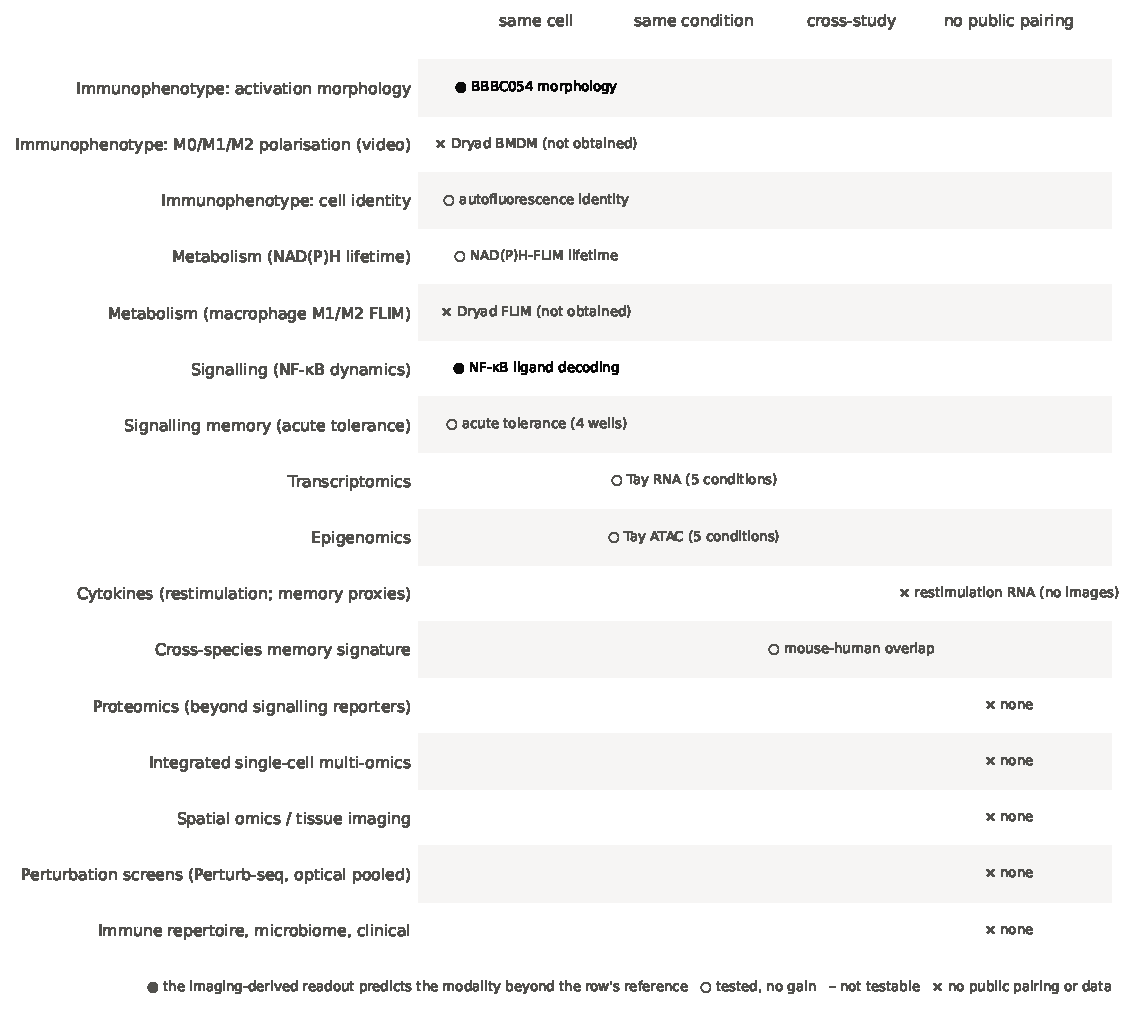
\includegraphics[width=\linewidth]{fig1_coverage_map.pdf}
\caption{Modality coverage map. Each row is a modality family; the column is the level at
which the best public dataset pairs it with images, video or image-derived dynamics of
innate immune cells. Filled circle: frozen image or dynamics features carry information
beyond the simple baseline of that row; open circle: tested, no such gain; cross: no
public pairing or data not obtainable. Details, numbers and sources in
Table~\ref{tab:coverage}.}
\label{fig:coverage}
\end{figure}}

\newcommand{\figtraining}{%
\begin{figure}[t]
\centering
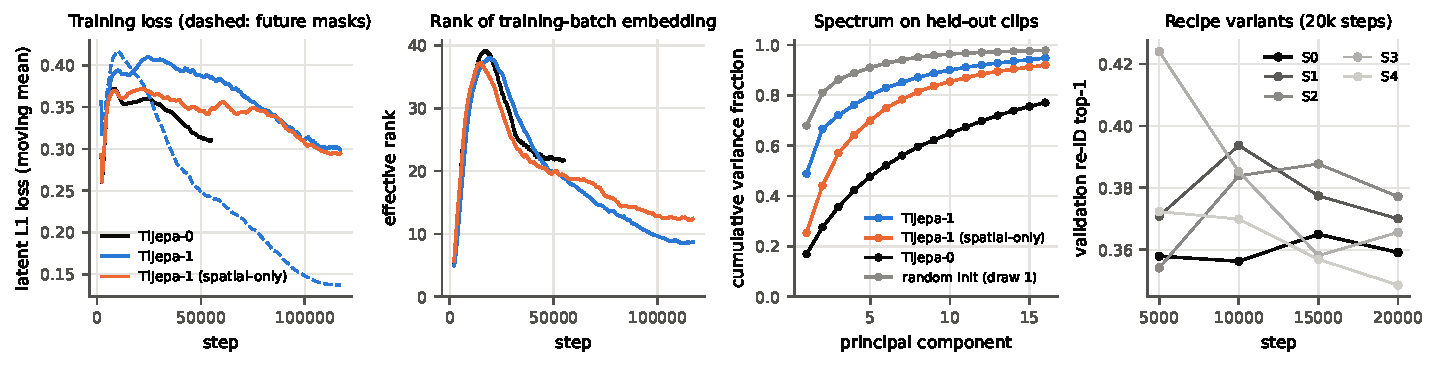
\includegraphics[width=\linewidth]{fig2_training_collapse.pdf}
\caption{Training and dimensional collapse. Left: latent loss of TiJepa-0, TiJepa-1 and
the spatial-only ablation (solid: spatially masked batches; dashed: future-masked batches).
Second: effective rank of the pooled target embedding of training batches (64 clips).
Third: cumulative variance of the leading principal components of the pooled target
embedding on held-out validation clips. Right: validation re-identification score of the
five 20,000-step recipe variants at each snapshot.}
\label{fig:training}
\end{figure}}

\newcommand{\figbenchmarks}{%
\begin{figure}[t]
\centering
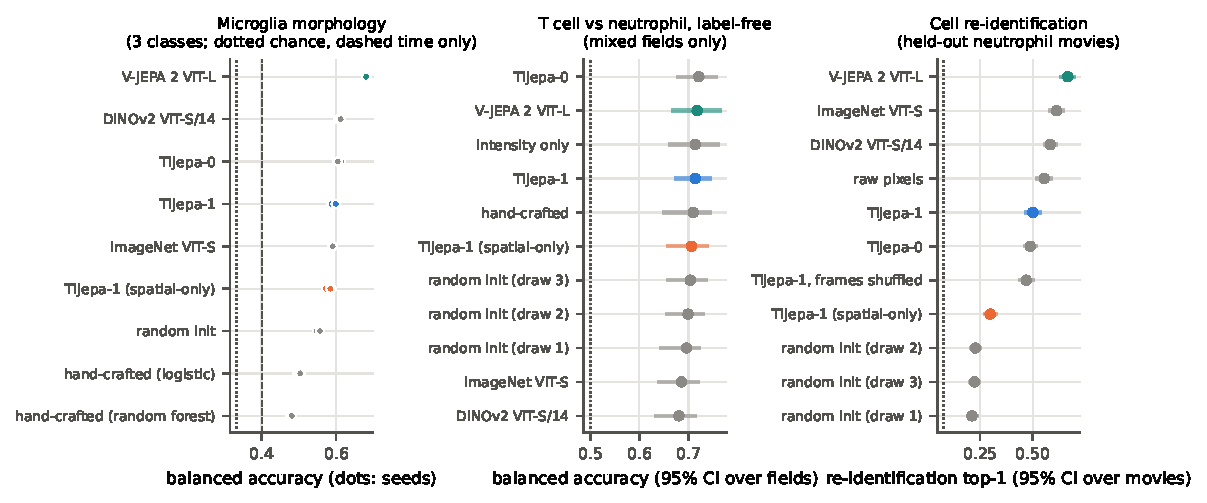
\includegraphics[width=\linewidth]{fig3_benchmarks.pdf}
\caption{Frozen-feature benchmarks. Left: microglia morphology (BBBC054), three-class
balanced accuracy, one dot per probe seed. Middle: T cells versus neutrophils from
label-free autofluorescence, on fields that contain both (95\% CI over fields). Right:
re-identification of the same neutrophil after 3--27 frames on held-out movies (95\% CI
over movies); this label-free validation set is the only data used to compare training
recipes.}
\label{fig:benchmarks}
\end{figure}}

\newcommand{\figassoc}{%
\begin{figure}[t]
\centering
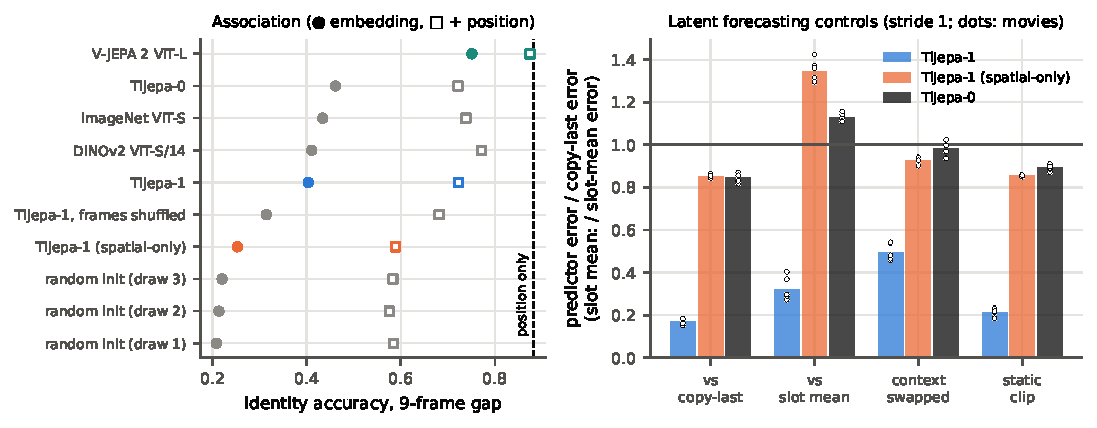
\includegraphics[width=\linewidth]{fig4_association_forecasting.pdf}
\caption{Association and forecasting. Left: identity matching of ground-truth cells across
a 9-frame gap from embedding distance alone (filled) and combined with centroid distance
(open); dashed line: centroid distance alone. Right: latent forecasting error relative to
copying the last context latent (first, third and fourth groups) or to the slot-conditional
mean fitted on other movies (second group), at stride 1; dots are movies. A forecasting
model should lose its advantage under a swapped context and on static clips; TiJepa-1 keeps
most of it.}
\label{fig:assoc}
\end{figure}}

\newcommand{\figsignalling}{%
\begin{figure}[t]
\centering
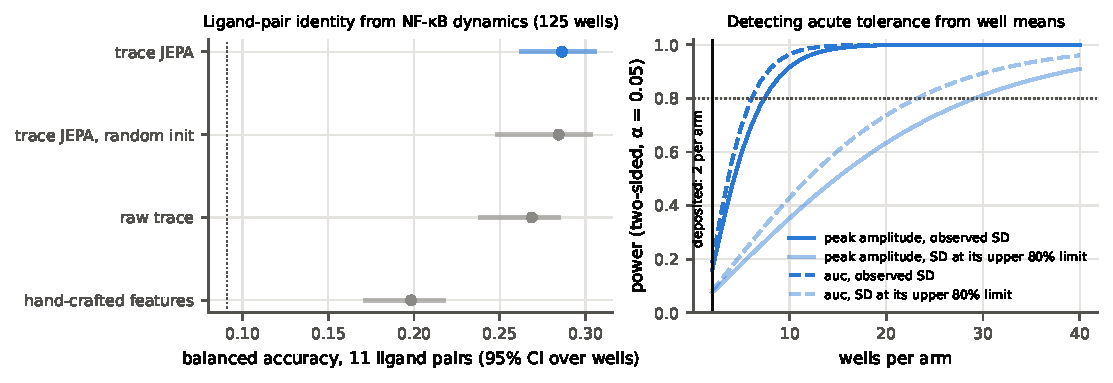
\includegraphics[width=\linewidth]{fig5_signalling.pdf}
\caption{NF-\(\kappa\)B dynamics. Left: decoding the ordered ligand pair from single-cell
traces (95\% CI over wells; dotted line: chance). Right: power of a well-level test for
acute tolerance as a function of wells per arm, at the observed effect (solid) and with the
between-well SD at the upper limit of its 80\% interval (faint).}
\label{fig:signalling}
\end{figure}}

\newcommand{\figrestim}{%
\begin{figure}[t]
\centering
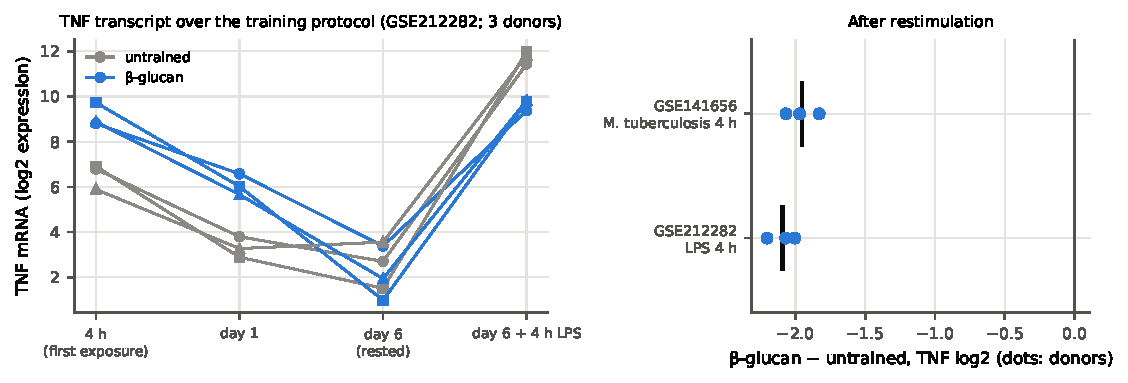
\includegraphics[width=\linewidth]{fig6_restimulation.pdf}
\caption{TNF transcripts in $\beta$-glucan-trained human macrophages. Left: TNF mRNA in
untrained (grey) and $\beta$-glucan-trained (blue) cells of three donors across the
training protocol of GSE212282; marker shape identifies the donor. Right: trained-minus-untrained TNF after 4\,h of
restimulation in two independent datasets; dots are donors, bars means.}
\label{fig:restim}
\end{figure}}

\newcommand{\figdesign}{%
\begin{figure}[t]
\centering
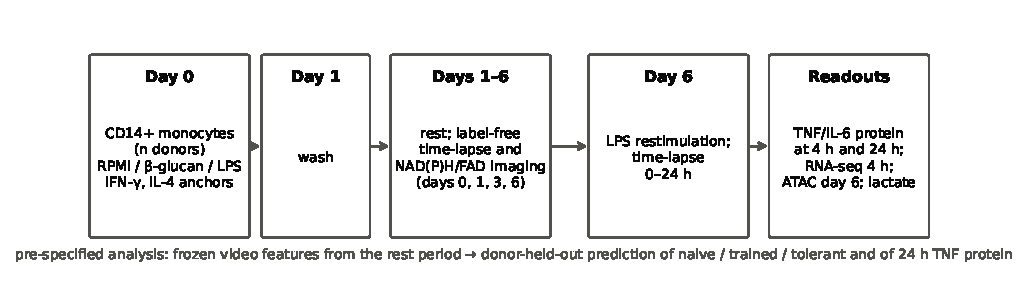
\includegraphics[width=\linewidth]{fig7_proposed_study.pdf}
\caption{The proposed imaging study of trained and tolerised human monocytes.}
\label{fig:design}
\end{figure}}

\newcommand{\CodeAvailability}{Code, configuration and the analysis records behind every
number are in the project repository, which will be linked here when it is made public.}

\title{Can imaging see innate immune memory? A public-data audit with a
self-supervised video model of innate-cell behaviour}

\author{\name Rafid Quadir \email rafidquadir@gmail.com}

\begin{document}
\maketitle

\begin{abstract}
Trained immunity and tolerance change how monocytes and macrophages respond to a second
stimulus, but they are measured by destructive restimulation assays. Whether these memory
states leave a signature that label-free imaging could read has not been tested, because no
public dataset images trained or tolerised cells. We asked how far public data can take the
question. We trained a self-supervised video model of innate-cell behaviour on
\val{pre.t1.clips} clips of migrating human neutrophils and tested it, with strong image and
video baselines, on every public dataset that pairs innate-cell imaging or live-cell dynamics
with a molecular, metabolic, signalling or functional readout, summarised as a modality
coverage map. Imaging features separate microglia activation morphologies, and NF-\(\kappa\)B
reporter dynamics encode stimulus identity, but frozen image features did not predict cell
identity or NAD(P)H lifetime beyond simple intensity statistics, and a general-purpose
video model outperformed the cell-specific one. Memory states themselves are paired with
imaging in no public resource. From the restimulation transcriptomes that do exist, after
sample-identity checks, we find that $\beta$-glucan-trained human macrophages have lower TNF
mRNA than untrained cells 4\,h after restimulation in two independent datasets (six of six
donors; \val{pc.212.tnf.d7.mean} and \val{pc.141.TNF.mean} log2), although the same studies
report higher TNF-$\alpha$ protein at 24\,h. A single readout time can therefore show
training as either enhanced or reduced, which shapes the imaging study we propose to test
innate immune memory directly.
\end{abstract}


\section{Introduction}
\label{sec:intro}
Innate immune cells keep a memory of earlier stimuli. Monocytes and macrophages exposed to
$\beta$-glucan or BCG respond more strongly to an unrelated second stimulus days later
(trained immunity), while cells exposed to LPS respond less (tolerance); both states are
carried by epigenetic and metabolic reprogramming rather than by antigen-specific receptors
\citep{netea2016,saeed2014,novakovic2016}. These states are measured today by restimulating
cells and assaying cytokines, transcripts or chromatin, which destroys the sample and gives
one time point. If memory states left a signature in how living cells look and move, label-free
video could read them out continuously and non-destructively.

Self-supervised video models make that question testable without labels: a joint-embedding
predictive architecture (JEPA) learns representations by predicting the latent content of
masked or future parts of a clip \citep{vjepa,vjepa2}. But testing whether such a model
captures immune state requires paired data, images or video of cells whose molecular or
functional state was measured, and for trained innate cells none is public. This paper asks
how far one can get with public data only. We train TiJepa, a video JEPA, on
\val{pre.t1.clips} unlabelled clips of migrating human neutrophils, and test its frozen
representations, against strong image and video models, on every public dataset we could
find that pairs label-free images, video or image-derived dynamics of innate immune cells with a
molecular, functional or memory readout.

The contribution is an audit rather than a new state of the art, and it has three parts.
\begin{enumerate}
\item A \emph{modality coverage map} (Figure~\ref{fig:coverage}, Table~\ref{tab:coverage}):
for each modality family (immunophenotype, metabolism, signalling, transcriptomics,
epigenomics, cytokines, integrated omics), the best public pairing with imaging, the level
at which it is paired (same cell, same condition, different studies), what we tested and
the result, including the families for which no public pairing exists.
\item A controlled evaluation of what a video JEPA learns from innate-immune video: a
matched-step spatial-only ablation, a frozen general-purpose video model (V-JEPA~2), image
models, random-initialisation and frame-shuffle controls, a label-free validation set used
for every model choice, controls that separate forecasting from positional structure in the
latent space, and a diagnosis of the partial dimensional collapse we observed.
\item From the molecular data that exist without images, a replicated observation that
constrains what an imaging study of trained cells should measure, and the design of that
study.
\end{enumerate}
Most of our answers are negative or null, and we report them as such. No result in this
paper shows trained immunity in images: no public image of trained cells exists, and the
memory-related analyses use the closest public proxies (acute priming and tolerance,
polarisation, restimulation transcriptomes).

\figcoverage
\section{Modality coverage map}
\label{sec:coverage}
Table~\ref{tab:coverage} and Figure~\ref{fig:coverage} summarise, for each modality family,
the best public pairing of innate immune cell imaging with that modality and what it
supports. Three things stand out. First, same-cell pairings exist only for
immunophenotype (morphology classes, cell type), metabolism (NAD(P)H lifetime) and
signalling (reporter dynamics), and none of them involves a memory state; the one
memory-adjacent same-cell resource, sequential NF-\(\kappa\)B stimulation, has two wells per
arm. Second, transcriptome and chromatin data are paired with dynamics only at the level of
five conditions, which supports description, not prediction. Third, the families in which
innate memory is actually measured, cytokines after restimulation and the transcriptional
and epigenetic programmes behind them, have no public imaging pairing at all; the
public restimulation transcriptomes (Section~\ref{sec:partC}) are what an imaging study of
memory would have to be validated against. Proteomics beyond signalling reporters,
integrated single-cell multi-omics, spatial omics, perturbation screens, repertoire,
microbiome and clinical data have no public pairing with in-vitro innate cell imaging.
For the same reason we did not project image features onto molecular activation axes: no
public dataset has both images and a stimulus-matched molecular anchor.

Within the same-cell pairings, frozen image or video features carry information about
morphology classes and NF-\(\kappa\)B dynamics carry information about stimulus identity, but
where a simple measured quantity is available as a reference (autofluorescence intensity
for cell identity; the photon-count image for lifetime), the learned features did not add
to it.

\begin{table}[t]
\centering
\scriptsize
\caption{Modality coverage map: the best public pairing of each modality family with images, video or image-derived dynamics of innate immune cells, what was tested and the result. BA: balanced accuracy.}
\label{tab:coverage}
\begin{tabular}{p{2.6cm}p{1.5cm}p{3.6cm}p{4.9cm}p{1.1cm}}
\toprule
Modality family & Pairing & Public data & Test and result & Outcome \\
\midrule
Immunophenotype: activation morphology & same cell & BBBC054 (mouse microglia, LPS time course; CC BY 3.0) & 3-class morphology from frozen features, FOV-grouped: best frozen encoder V-JEPA 2 ViT-L BA 0.681 vs hand-crafted 0.499; TiJepa-1 0.595 & positive \\
Immunophenotype: M0/M1/M2 polarisation (video) & same cell & Dryad m0cfxpp8v (BMDM movies) & polarisation from frozen video features: not obtained: the download requires an interactive browser check & absent \\
Immunophenotype: cell identity & same cell & Zenodo 15657646 (two-photon autofluorescence, T cells and neutrophils in the same fields; CC BY 4.0) & T cell vs neutrophil, FOV-grouped, mixed fields only: best frozen encoder TiJepa-0 BA 0.721; intensity-only baseline 0.714 (CI 0.663-0.760) & null \\
Metabolism (NAD(P)H lifetime) & same cell & Zenodo 14330511 (two-photon NAD(P)H-FLIM, macrophages; CC BY 4.0) & per-cell mean lifetime from the photon-count image, FOV-grouped ridge: best frozen encoder TiJepa-1 (spatial-only) $R^2$ +0.32; intensity baseline +0.12; knowing only the experimental arm +0.50; within fields: TiJepa-1 +0.08, intensity +0.08 & null \\
Metabolism (macrophage M1/M2 FLIM) & same cell & Dryad 8gtht76q2 & not obtained: the download requires an interactive browser check & absent \\
Signalling (NF-$\kappa$B dynamics) & same cell & Tay lab deposit, Zenodo 14337874 (live-cell NF-$\kappa$B reporter, 125 wells) & 11-way ligand-pair identity from single-cell traces, well-grouped: trace JEPA BA 0.286, raw trace 0.269, hand-crafted 0.198; reference: chance 0.091. Pretraining adds nothing over the same network at random initialisation & positive \\
Signalling memory (acute tolerance) & same cell & Tay deposit, LPS then LPS (4 wells) & tolerant vs naive from the second response; power analysis: unpowered (2 wells per arm); 8 wells per arm needed for 80\% power at the observed effect & null \\
Transcriptomics & same condition & Tay RNA-seq GSE260996 (same lab as the imaging; 5 conditions) & condition-level dynamics $\to$ RNA ($Q^2$ vs leave-one-out mean): fraction of top-2,000 genes with $Q^2$ > 0: 0.226 (exact permutation p 0.36; 5 conditions, descriptive) & null \\
Epigenomics & same condition & Tay ATAC-seq GSE261647 (5 conditions) & condition-level dynamics $\to$ accessibility: fraction of top-2,000 peaks with $Q^2$ > 0: 0.182 (exact permutation p 0.44; 5 conditions, descriptive) & null \\
Cytokines (restimulation; memory proxies) & no public pairing & GSE212282, GSE185433, GSE141656 (human macrophage training and tolerance, RNA only; no images) & TNF/IL6 transcripts after restimulation, donor-paired: $\beta$-glucan-trained cells: TNF transcript lower at 4 h after LPS (3/3 donors) and after M. tuberculosis (3/3, independent donors) & absent \\
Cross-species memory signature & cross-study & Tay mouse RNA (priming x LPS) vs GSE185433 human tolerance & overlap of priming-blunted LPS genes among genes induced in both species: overlap 18 vs 24.5 expected, OR 0.58, two-sided p 0.09 & null \\
Proteomics (beyond signalling reporters) & no public pairing & - & no public dataset pairs images of innate immune cells with proteomics & absent \\
Integrated single-cell multi-omics & no public pairing & - & no public dataset pairs live-cell imaging of innate cells with single-cell multi-omics of the same cells & absent \\
Spatial omics / tissue imaging & no public pairing & - & in-tissue data exist but not for the in-vitro cell systems studied here & absent \\
Perturbation screens (Perturb-seq, optical pooled) & no public pairing & - & no public optical or Perturb-seq screen of trained or tolerised innate cells & absent \\
Immune repertoire, microbiome, clinical & no public pairing & - & not applicable to in-vitro innate-cell imaging & absent \\
\bottomrule
\end{tabular}
\end{table}

\section{What restimulation transcriptomes say that imaging would need to detect}
\label{sec:partC}
No public dataset images trained or tolerised monocytes, but three public datasets measure
their transcripts after restimulation. We use them to ask which differences an imaging
study would have to reproduce, with three safeguards: every restimulation label is checked
against the GEO sample records and against a positive control (restimulated untrained
cells must exceed unstimulated untrained cells for TNF, IL6 and IL1B in every donor), every
expected direction is quoted from the dataset's source publication, and sample identity is
verified before any observation is reported.

\paragraph{Sourced directions.} Of the \val{pc.v2.n_sourced} TNF and IL-6 directions the
source publications report after restimulation, \val{pc.v2.n_match} agree in sign with the
mean donor-paired difference in the deposited transcripts: dimethyl itaconate (GSE212282) and IL-4 (GSE185433)
increase TNF and IL6 transcripts, as their source papers report for the secreted proteins
\citep{ferreira2023,schrijver2023}. The two exceptions are both $\beta$-glucan.

\paragraph{$\beta$-glucan lowers the TNF transcript at 4\,h after restimulation, in two
independent datasets.} In GSE212282, $\beta$-glucan-trained macrophages restimulated with LPS
for 4\,h on day 6 have less TNF mRNA than untrained cells in all three donors (log2
difference \val{pc.212.tnf.d7.min} to \val{pc.212.tnf.d7.max}), although the source paper
reports more secreted TNF-$\alpha$ after 24\,h of restimulation
\citep{ferreira2023}. Before reporting this we checked sample identity. All
\val{qc.212.n} samples agree on sex within each donor; the three donors carry distinct
presence/absence genotypes at HLA-DRB5 and GSTM1, consistent across every sample of a donor,
so no sample belongs to another donor; and after removing each donor's mean, every
$\beta$-glucan sample's profile is most similar to the other donors' $\beta$-glucan samples
(day-6 restimulated arms: \val{qc.212.d7.match} samples matched to their own arm, the one
exception being a $\beta$-glucan + DMI sample matched to DMI). Over the protocol the
$\beta$-glucan effect on TNF reverses: it raises the transcript during the first exposure
(4\,h: \val{pc.212.tnf.4H.min} to \val{pc.212.tnf.4H.max}; day 1: \val{pc.212.tnf.d1.min} to
\val{pc.212.tnf.d1.max}), is inconsistent at rest on day 6 (\val{pc.212.tnf.d6.min} to
\val{pc.212.tnf.d6.max}) and lowers it after restimulation (Figure~\ref{fig:restim}).

The observation replicates in GSE141656, an independent dataset none of whose three donors
matches a GSE212282 donor at all four genotype-like loci we compared: after 4\,h of heat-killed \emph{M. tuberculosis}
on day 6, $\beta$-glucan-trained macrophages have less TNF mRNA in every donor
(\val{pc.141.TNF.min} to \val{pc.141.TNF.max}; restimulation positive control at least
\val{pc.141.pc.tnf.min} log2 units in every donor), and IL6 (\val{pc.141.IL6.mean}) and
IL1B (\val{pc.141.IL1B.mean}) move the same way. Its source publication, too, reports more
TNF-$\alpha$ protein after 24\,h of restimulation \citep{moorlag2020}. A third dataset with
only two replicates (GSE242947, \citealp{cheng2024dectin}) is consistent at 1\,h of LPS
(\val{pc.242.tnf.1h}) and inconsistent at 3\,h (\val{pc.242.tnf.3h}).

We therefore report a replicated, transcript-level observation: at 4\,h after
restimulation, $\beta$-glucan-trained human macrophages have lower TNF mRNA than untrained
ones, in two datasets and six donors, while the same studies report higher TNF-$\alpha$
protein at 24\,h. One explanation is kinetic, that trained cells reach their TNF transcript
peak earlier and resolve it sooner; it is a hypothesis, and the test is a restimulation time
course from 0.5 to 24\,h with paired RNA and protein. With three donors per dataset no
confidence interval is reported; the smallest achievable exact $p$ for a three-donor
sign-flip test is 0.25, so the evidence is the consistency across six of six donors and two
restimuli, not a $p$-value.

\figrestim
\section{Signalling dynamics: what live-cell traces encode}
\label{sec:partB}
The Tay-lab deposit \citep{wang2025} is the one public resource in which live-cell
dynamics of macrophages, here single-cell NF-\(\kappa\)B reporter traces, are paired at the
condition level with transcriptome and chromatin data, and it includes sequential
stimulations, which is the structure innate memory has.

\paragraph{Ligand-pair identity is decodable from dynamics.} Across \val{pb.lig.wells}
wells and \val{pb.lig.n} cells, the identity of the ordered pair of stimuli
(\val{pb.lig.classes} classes, chance \val{pb.lig.chance}) is decoded from single-cell
traces well above chance, with wells as groups (Figure~\ref{fig:signalling}): the raw trace
reaches \val{pb.lig.raw_trace} (95\% CI \val{pb.lig.raw_trace.ci}), hand-crafted trace
features \val{pb.lig.handcrafted} (\val{pb.lig.handcrafted.ci}), and a trace JEPA, pretrained
without labels on \val{pb.pre.cells} traces from \val{pb.pre.wells} wells that are not
evaluated, \val{pb.lig.trace_jepa} (\val{pb.lig.trace_jepa.ci}). The pretraining is not
what helps: the same network at random initialisation reaches
\val{pb.lig.trace_jepa_random_init} (difference \val{pb.lig.d.trace_jepa_random_init},
95\% CI \val{pb.lig.d.trace_jepa_random_init.ci}), and its advantage over the raw trace
(\val{pb.lig.d.raw_trace}, \val{pb.lig.d.raw_trace.ci}) does not survive correction for
multiple comparisons. Hand-crafted summaries lose information that the full trace carries
(\val{pb.lig.d.handcrafted}, \val{pb.lig.d.handcrafted.ci}).

\paragraph{Acute tolerance cannot be tested with the deposited wells.} The deposit has two
wells of LPS-then-LPS and two of naive-then-LPS cells, so a well-level test of tolerance
from dynamics has no power. From the observed well means of the second response's peak
amplitude (standardised effect \val{pb.pow.peak_amplitude.d}) and their between-well SD, a
two-sided test at $\alpha=0.05$ needs \val{pb.pow.peak_amplitude.n} wells per arm for 80\%
power, and \val{pb.pow.peak_amplitude.nhi} if the SD is at the upper limit of its 80\%
interval; for the response's area under the curve the numbers are \val{pb.pow.auc.n} and
\val{pb.pow.auc.nhi}. Because that SD rests on four wells, we read this as a lower bound on
what a tolerance-from-dynamics study needs, not as a precise design.

\paragraph{Dynamics to omics and across species.} With five matched conditions, condition-
level dynamics do not predict held-out transcript or accessibility profiles better than the
leave-one-out mean (Table~\ref{tab:coverage}), and among \val{b4.both.uni} orthologs induced
by LPS in both mouse macrophages and human macrophages, the genes blunted by heterologous
priming in mouse overlap the genes blunted by homologous tolerance in human no more than
expected by chance (\val{b4.both.k} observed, \val{b4.both.exp} expected, odds ratio
\val{b4.both.or}, two-sided $p=\val{b4.both.p}$). Both analyses are exploratory.

\figsignalling
\section{What a video JEPA learns from innate-immune video}
\label{sec:partA}

\subsection{Morphology of activated microglia}
On BBBC054, every learned representation separates the three microglia morphology classes
far better than hand-crafted shape and texture features (\val{bb.E1_handcrafted_logreg.3c})
or exposure time alone (\val{bb.time.3c}; Figure~\ref{fig:benchmarks}). The pretrained
video model V-JEPA~2 is the best encoder (\val{bb.E7_vjepa2_vitl.3c}). TiJepa-1
(\val{bb.E4_tijepa1.3c}) is not distinguishable from DINOv2 (\val{bb.E3_dinov2_vit_s.3c}),
the ImageNet ViT (\val{bb.E2_imagenet_vit_s.3c}) or TiJepa-0 (\val{bb.E0_tijepa0.3c});
V-JEPA~2 exceeds it by \val{bb.d.E4_tijepa1.E7_vjepa2_vitl.3c.abs} (95\% CI
\val{bb.ci.E4_tijepa1.E7_vjepa2_vitl.3c.abs}). Training on cell video therefore did not beat a
general-purpose video model, and twice as many training steps on a quality-filtered corpus
did not improve on TiJepa-0. Within the TiJepa recipe, future masking adds
\val{bb.d.E4_tijepa1.E4s_tijepa1_spatial.3c}
(\val{bb.ci.E4_tijepa1.E4s_tijepa1_spatial.3c}) over the spatial-only ablation and training
adds \val{bb.d.E4_tijepa1.E6_random_init.3c} (\val{bb.ci.E4_tijepa1.E6_random_init.3c})
over a randomly initialised network of the same architecture, which itself reaches
\val{bb.E6_random_init.3c}. In the round-versus-amoeboid task the ordering is the same at a
higher level (V-JEPA~2 \val{bb.E7_vjepa2_vitl.ra}, TiJepa-1 \val{bb.E4_tijepa1.ra}, DINOv2
\val{bb.E3_dinov2_vit_s.ra}). Accuracy depends on apparent cell size: rescaling the crops
by 0.5, 0.75, 1 and 1.5 before encoding gives \val{bb.scale.0.5}, \val{bb.scale.0.75},
\val{bb.scale.1.0} and \val{bb.scale.1.5} for TiJepa-1, so differences in magnification
between pretraining and evaluation data matter.

\subsection{Label-free cell identity}
On T cells and neutrophils imaged in the same fields, frozen encoders reach balanced
accuracies of \val{af.Am.frozen.min}--\val{af.Am.frozen.max} on the \val{af.Am.fovs}
mixed fields, every one of them inside the 95\% CI of a probe on per-channel intensity
statistics (\val{af.Am.intensity_baseline.all}, CI \val{af.Am.intensity_baseline.all.ci};
Figure~\ref{fig:benchmarks}). TiJepa-1 reaches
\val{af.Am.E4_tijepa1.all} and V-JEPA~2 \val{af.Am.E7_vjepa2_vitl.all}; random
initialisation reaches \val{af.Am.E6_random_init_draw0.all}. On the gradient-contrast
channel alone, which is closest to the brightfield TiJepa was trained on, TiJepa-1 gives
\val{af.Am.E4_tijepa1.dodt} and V-JEPA~2 \val{af.Am.E7_vjepa2_vitl.dodt}. Cell identity in
these data is carried by autofluorescence intensity; frozen image features add nothing measurable
to it. In the six-class set, where each cell type was imaged in its own session, the
hand-crafted features reach \val{af.B.E1_handcrafted.all} and TiJepa-1
\val{af.B.E4_tijepa1.all}; that comparison cannot separate cell type from session.

\subsection{NAD(P)H lifetime from the photon image}
In \val{fl.cells} macrophages from \val{fl.fovs} fields, the per-cell mean NAD(P)H lifetime
(\val{fl.tau.mean}\,$\pm$\,\val{fl.tau.sd}\,ns; our data check required a median between
0.3 and 3.5\,ns)
is predicted from frozen features of the photon-count image with $R^2$ up to
\val{fl.tau.E4s_tijepa1_spatial} (TiJepa-1 \val{fl.tau.E4_tijepa1}, V-JEPA~2
\val{fl.tau.E7_vjepa2_vitl}), against \val{fl.tau.intensity_baseline} for intensity statistics.
That gain does not reflect cell-level metabolism. Lifetime differs between experimental
arms, and a reference that predicts each cell by its arm's training-fold mean reaches
$R^2=\val{fl.ref.tau}$, more than any image feature. When targets and features are centred
on their field's mean, so that only variation between cells of one field counts, TiJepa-1
reaches \val{fl.wf.tau.E4_tijepa1} (95\% CI \val{fl.wf.tau.E4_tijepa1.ci}), V-JEPA~2
\val{fl.wf.tau.E7_vjepa2_vitl} and intensity statistics \val{fl.wf.tau.intensity_baseline}
(\val{fl.wf.tau.intensity_baseline.ci}); the bound fraction behaves the same way. These two
controls were added after seeing the first result. The frozen features recognise the
condition a field came from; they do not read a cell's lifetime beyond its brightness.

\subsection{Forecasting is explained by positional structure}
\label{sec:forecasting}
TiJepa-1's predictor forecasts its own future latents with an error \val{fc.E4_tijepa1.1.ratio_vs_copy_last}
times that of copying the last context latent, against \val{fc.E4s_tijepa1_spatial.1.ratio_vs_copy_last}
for the spatial-only ablation, which never saw a future mask, and the advantage holds at
every stride (Figure~\ref{fig:assoc}). It also beats a slot-conditional mean fitted on other
movies (ratio \val{fc.E4_tijepa1.1.ratio_vs_slot_mean}, exact $p=\val{fc.E4_tijepa1.1.p.slot}$,
the smallest possible with six movies), so its predictions are specific to the clip. But
the controls show that the advantage over copy-last is not evidence of modelling cell
dynamics. On static clips, in which nothing moves, the predictor keeps
\val{fc.E4_tijepa1.1.adv.static} of its \val{fc.E4_tijepa1.1.adv} improvement over
copy-last; given the context of a different clip from the same movie it keeps
\val{fc.E4_tijepa1.1.adv.swap}. Copy-last is a weak reference because the target encoder's
latents change with temporal position even when the image does not, and the predictor
receives those positions. Decoded to pixels, the predictions are no closer to the future
frames than the last observed frame (error ratio \val{fc.E4_tijepa1.1.pixel_ratio_decoded_pred_vs_pixel_copy_last}
at stride 1, \val{fc.E4_tijepa1.27.pixel_ratio_decoded_pred_vs_pixel_copy_last} at stride
27). Our pre-specified criterion for forecasting \val{fc.pass}, and we make no forecasting
claim.

\subsection{Re-identifying cells over time}
\label{sec:reid}
On the \val{val.movies} held-out validation movies, re-identifying the same cell after 3 to
27 frames among all cells at that time (chance \val{re.chance}) separates the encoders
clearly (Figure~\ref{fig:benchmarks}). V-JEPA~2 is best (\val{re.E7_vjepa2_vitl}, 95\% CI
\val{re.E7_vjepa2_vitl.ci}), followed by the ImageNet ViT (\val{re.E2_imagenet_vit_s}) and
DINOv2 (\val{re.E3_dinov2_vit_s}); raw downsampled pixels reach \val{re.raw_pixels}
(\val{re.raw_pixels.ci}). TiJepa-1 reaches \val{re.E4_tijepa1} (\val{re.E4_tijepa1.ci}),
below raw pixels. Among TiJepa models the training objective matters: the spatial-only
ablation reaches only \val{re.E4s_tijepa1_spatial} (\val{re.E4s_tijepa1_spatial.ci}), and
randomly initialised networks \val{re.E6_random_init_draw0}--\val{re.E6_random_init_draw1}.
Shuffling the frames of TiJepa-1's input clips lowers its score to \val{re.E5_frame_shuffled},
so it uses the order of frames only slightly. Because this set is used to compare training
recipes, these numbers describe the models; they are not a held-out test.

\subsection{Dimensional collapse}
\label{sec:collapse}
The effective rank of TiJepa-1's pooled embedding on a fixed set of microglia crops fell
from \val{mon.t1.rank.first} at step 14{,}751 to \val{mon.t1.rank.last} at the end of
training, and its per-dimension standard deviation from \val{mon.t1.std.first} to
\val{mon.t1.std.last}; the spatial-only ablation ended at \val{mon.ts.rank.last}
(Figure~\ref{fig:training}). The collapse is a property of the encoder, not of the probe
input: on held-out validation clips the pooled target-encoder and context-encoder embeddings
of TiJepa-1 have the same effective rank (\val{dg.E4_tijepa1.target.rank} and
\val{dg.E4_tijepa1.context.rank} of 384), the first principal component carries
\val{dg.E4_tijepa1.target.top1} of the variance and the first eight
\val{dg.E4_tijepa1.target.top8}. Individual tokens are less collapsed (effective rank
\val{dg.E4_tijepa1.token.rank}), so the information lost is mostly in what survives mean
pooling. TiJepa-0's pooled embedding has rank \val{dg.E0_tijepa0.target.rank} on the same
clips. Across the six pretrained and random networks, effective rank on the validation
clips is correlated with both the microglia accuracy (Spearman $\rho=\val{dg.rho.bb}$) and
the re-identification score ($\rho=\val{dg.rho.val}$), which is descriptive with six
models. In the training logs the rank of the training-batch embedding peaks within the first
20{,}000 steps and declines while the EMA momentum rises towards 1 and the learning rate
decays, so the cause cannot be separated from the schedule without changing the recipe;
Section~\ref{sec:recipe} reports a short recipe study that does so.

\figbenchmarks
\figassoc
\figtraining
\section{Discussion}
\label{sec:discussion}
\paragraph{What the video JEPA learned.} Trained on \val{pre.t1.clips} clips of one cell type
from one instrument, TiJepa-1 learned representations that classify microglia morphology
far better than hand-crafted features. Image models trained on millions of natural images
do as well, and a general-purpose video model used frozen and off the shelf, V-JEPA~2,
does better. On the label-free validation task TiJepa-1 is below raw pixels.
Future masking helps relative to the matched spatial-only ablation, modestly on morphology
and strongly on re-identification, but the predictor's apparent forecasting skill is
explained by the positional structure of its own target latents: it persists on clips in
which nothing moves. The representation is partially collapsed, and rank and downstream
performance move together across models. A practitioner who wants frozen features of
innate-cell video today should start from a large pretrained video model.

\paragraph{What public data can and cannot answer.} The coverage map makes the central gap
concrete: every public pairing of innate-cell imaging with a molecular or functional readout
is either at the same-cell level for states that are not memory (morphology classes, cell
type, metabolic lifetime, stimulus identity), or at the condition level with five conditions.
Where a simple measured reference exists (autofluorescence intensity for cell identity,
the photon image for lifetime) the learned features did not add to it. The memory states
themselves are measured only by restimulation assays that have never been imaged.

\paragraph{A constraint for the experiment that is missing.} The replicated observation
that $\beta$-glucan-trained human macrophages have less TNF transcript than untrained cells
4\,h after restimulation, in two datasets with different restimuli and donors, while the
same studies report more TNF-$\alpha$ protein at 24\,h, means that a single readout time can
show training as either enhanced or reduced. An imaging study of trained immunity therefore
needs its molecular ground truth at more than one time after restimulation, and its
imaging window should cover the hours in which the transcript and protein responses
diverge (Section~\ref{sec:future}).

\subsection{Future work: the experiment that would test this directly}
\label{sec:future}
No public dataset images trained or tolerised human monocytes, so whether innate immune
memory has an imaging phenotype remains untested. The study that would test it
(Figure~\ref{fig:design}) uses primary human CD14$^+$ monocytes from independent donors in
five arms: medium, $\beta$-glucan (training), LPS (tolerance), and IFN-$\gamma$ and IL-4 as
polarisation anchors with known morphological and metabolic effects. Cells are exposed for
24\,h, washed and rested for 5 days, then restimulated with LPS on day 6. Label-free
brightfield time-lapse is recorded during the rest and for 0--24\,h after restimulation, at a
frame interval chosen to cover the horizons our forecasting analysis spanned (8\,s to
3.6\,min); NAD(P)H/FAD autofluorescence, with lifetime imaging where available, is acquired
on days 0, 1, 3 and 6. Ground truth is TNF and IL-6 protein at 4\,h and 24\,h after
restimulation, bulk RNA-seq at 4\,h, ATAC-seq on day 6 and lactate in the supernatant.

The analysis is fixed in advance: frozen video features (TiJepa, DINOv2 and V-JEPA~2) of
the rest-period movies, donor-held-out classification of naive, trained and tolerised wells,
and donor-held-out prediction of 24\,h TNF protein from pre-restimulation video, with
image-free baselines (well-level intensity and cell counts) as the reference; the primary
endpoint is the gain over that reference. The hypothesis is falsified if no frozen feature set
exceeds the reference with a donor-level confidence interval excluding zero. Effects
between donors are consistent in the transcript data (the SD of the trained-minus-untrained
TNF difference after restimulation is \val{ds.tnf.sd212} and \val{ds.tnf.sd141} log2 units
in the two datasets), but nothing constrains the size of an imaging effect. Assuming a
standardised donor-level effect of 1.0 (0.8, 1.5), a paired two-sided test at
$\alpha = 0.05$ needs \val{ds.n.d1.0} (\val{ds.n.d0.8}, \val{ds.n.d1.5}) donors for 80\%
power. Images would be deposited in the BioImage Archive under CC~BY, sequencing in GEO,
and cytokine and plate metadata alongside.

\figdesign
\section{Limitations}
\label{sec:limitations}
\paragraph{Cell types.} The model is pretrained on human neutrophil migration, evaluated on
neutrophils, mouse microglia, mouse immune cells and FLIM-imaged macrophages, and the
memory biology concerns human monocyte-derived macrophages. Every transfer across that
chain is an assumption the data cannot check; the activation-labelled macrophage movies
that would have tested it directly could not be obtained.

\paragraph{Seeds and scale.} One pretraining seed was run per recipe on one GPU, so
differences between pretrained models carry no seed-to-seed uncertainty; the probe seeds
reported vary only the folds and subsamples. TiJepa is a ViT-S trained for about
\val{pre.t1.gpuh} GPU-hours on a single-source corpus; V-JEPA~2 is a ViT-L trained on
orders of magnitude more video.

\paragraph{Collapse.} Feature effective rank fell throughout training for every recipe we
trained to completion (Section~\ref{sec:collapse}); our 20{,}000-step recipe study
(Section~\ref{sec:recipe}) ends before the collapse sets in and does not establish its cause.

\paragraph{Small groups.} Six tracking movies, four tolerance wells, five matched omics
conditions and three donors per restimulation dataset are below the size at which we
report confidence intervals; those analyses give per-group values and exact tests, and the
tolerance and dynamics-to-omics analyses are descriptive.

\paragraph{Readouts.} The restimulation observation is at the transcript level at 4\,h; the
24\,h protein results it contrasts with are those reported by the source publications, not
re-measured. The NAD(P)H lifetime readouts are computed without deconvolving the
instrument response and are relative measures.

\section{Related work}
\label{sec:related}
\paragraph{Self-supervised video representation learning.}
JEPA-style video models predict masked spatio-temporal regions in latent space rather than
pixels \citep{vjepa}; V-JEPA~2 scales the approach to over a million hours of video and adds
action-conditioned prediction \citep{vjepa2}. Image self-supervision (DINOv2,
\citealp{dinov2}) and supervised ImageNet ViTs \citep{augreg} are the usual frozen
baselines. Variance and covariance regularisation counteracts
dimensional collapse in joint-embedding training \citep{vicreg}.

\paragraph{Label-free imaging of immune cell state.}
Label-free two-photon autofluorescence of NAD(P)H and FAD has been used to classify immune
cell types \citep{kreiss2026cellmics}, and NAD(P)H lifetime imaging reports the metabolic
state of macrophages \citep{musimbi2025flim}. High-throughput migration imaging of
neutrophils in multi-well plates is available at scale \citep{complexeye}. Live-cell
NF-\(\kappa\)B reporter dynamics of macrophages exposed to sequential ligand pairs have been
deposited together with transcriptome and chromatin measurements of the same conditions
\citep{wang2025}.

\paragraph{Innate immune memory.}
Trained immunity and tolerance are defined functionally by the response to restimulation
\citep{netea2016} and are accompanied by epigenetic and transcriptional reprogramming of
monocytes and macrophages \citep{saeed2014,novakovic2016}. Public restimulation datasets
measure transcripts and, in their source publications, secreted cytokines
\citep{ferreira2023,schrijver2023,moorlag2020}; none includes images.

% Methods shared by both versions. Numbers come from numbers.tex (\val{...}).
\section{Methods}
\label{sec:methods}

\subsection{Pretraining data}
\label{sec:corpus}
The pretraining corpus consists of label-free brightfield time-lapse movies of human
neutrophils migrating in multi-well plates, from the ComplexEye deposit
\citep{complexeye} (Zenodo 10082674, CC BY 4.0). Ten of the deposit's 21
archives were used. Every movie was checked for duplication against the held-out
tracking movies before use (Section~\ref{sec:leakage}), passed a per-frame focus and
illumination check, was kept at its native pixel size (0.641\,\textmu m/px, within 1.5\%
of the 0.65\,\textmu m/px target), and was cut into cell-centred clips of 16 frames of
$96\times96$ pixels that follow a tracked cell. Clips were taken at temporal strides of 1,
3, 9 and 27 frames (frame interval 8\,s, so a clip spans 2\,min to 60\,min), and 10\% of
clips were replaced by a single frame repeated 16 times so that the model also sees static
input. The frozen corpus holds \val{pre.t1.clips} clips from 407 movies; its index and
shards are fixed by checksum, and every model below was trained on exactly this set.

\subsection{Model}
TiJepa is a video joint-embedding predictive architecture
\citep{vjepa}. A ViT-S encoder (12 layers, width 384, 6 heads) embeds
$2\times8\times8$ tubelets of a $16\times96\times96$ single-channel clip into an
$8\times12\times12$ token grid with fixed 3-D sine-cosine positional embeddings. A context
encoder sees only the visible tokens; a target encoder, an exponential moving average
(EMA) of the context encoder, sees the full clip; a 6-layer predictor of width 192
receives the context tokens and the positional embeddings of the masked positions and
predicts the target encoder's layer-normalised tokens there, with an L1 loss. Each batch
uses one of two masks: with probability 0.5 a \emph{future} mask that hides every spatial
position of the last two temporal slots (the last 4 frames), otherwise a spatial tube mask
of 8 random blocks spanning all frames. The \emph{spatial-only} ablation uses only the
second mask. Representations for every downstream task are the mean-pooled tokens of the
frozen target encoder.

\subsection{Training}
Both TiJepa-1 and its spatial-only ablation were trained from scratch for
\val{pre.t1.steps} steps of batch 128 (\val{pre.t1.epochs} passes over the corpus) with
AdamW (learning rate $1.5\times10^{-4}$ after 500 warm-up steps, cosine decay to 0, weight
decay 0.05, $\beta=(0.9, 0.95)$), bf16 autocast and gradient clipping at 1.0; the EMA
momentum rose linearly from 0.996 to 1.0. Both schedules end exactly on the last step.
TiJepa-1 used \val{pre.t1.gpuh} and the ablation \val{pre.ts.gpuh} A100-40GB GPU-hours.
TiJepa-1 was trained in two segments, resumed from a checkpoint with its data stream,
masks and optimiser state restored. We also report TiJepa-0, an earlier model trained for
55{,}000 steps with spatial masking only on a smaller corpus from 7 archives without the
quality filter; it is a historical reference, not an ablation, because its corpus differs.
One pretraining seed was run per recipe.

\subsection{Frozen baselines}
All encoders are frozen; only linear probes are fitted. Baselines are an ImageNet-trained
ViT-S/16 \citep{augreg}, DINOv2 ViT-S/14 \citep{dinov2}, the
general-purpose video model V-JEPA~2 ViT-L \citep{vjepa2} (MIT licence;
Hugging Face \texttt{facebook/vjepa2-vitl-fpc64-256} at a pinned revision), the same
TiJepa architecture at random initialisation (three independent draws), TiJepa-1 with the
frames of each clip shuffled, and dataset-specific hand-crafted features. Grayscale input
is replicated to three channels for image and video models and resized to each model's
native resolution with its own normalisation; still images are repeated over 16 frames for
video models. Image models see the last frame of a clip.

\subsection{Evaluation protocol}
\label{sec:protocol}
Every probe is fitted with group-held-out cross-validation, where the group is the unit
of acquisition (field of view, movie, well or donor), so no group contributes to both the
training and the test folds. Unless stated otherwise the probe is standardisation,
PCA to 64 dimensions and class-balanced logistic regression (ridge regression for
continuous targets), with three seeds that vary the fold assignment and, where the data
are subsampled, the subsample. We report balanced accuracy (BA) or $R^2$. Confidence
intervals are 95\% cluster bootstraps over groups (2{,}000 resamples) and are reported
only with at least 10 groups; comparisons between encoders are paired bootstraps on the
same resamples with Benjamini--Hochberg correction within a task. With fewer than 10
groups we report every group's value and exact sign-flip or permutation tests, whose
smallest achievable $p$ is stated. Model and recipe choices were made only on a
label-free validation set that is never used for any reported result
(Section~\ref{sec:validation}); every reported number comes from a model frozen before its
test set was used. Every result records the checkpoint (file, step, SHA-256) it came from,
and every model name in this paper is derived from that record.

\subsection{Leakage control}
\label{sec:leakage}
Every corpus movie was fingerprinted (block-averaged frames at the start, middle and end)
and compared with the six held-out tracking movies; candidate pairs were re-tested at full
resolution. One corpus movie duplicated a held-out movie and was excluded from the corpus;
TiJepa-0's older corpus contained it, so that movie is dropped from every TiJepa-0
tracking summary. The validation movies were checked against both the held-out movies and
the corpus (Section~\ref{sec:validation}).

\subsection{Benchmarks}
\paragraph{Validation: cell re-identification.}
\label{sec:validation}
Sixty-four movies from a ComplexEye archive that is not in the corpus form the validation
set. Cells were detected and linked with the same classical pipeline used to build the
corpus. At four anchor frames per movie, every cell tracked without gaps from 15 frames
before to 42 frames after the anchor is embedded from the 16-frame clip ending at the
anchor (the query) and from the clip starting $k\in\{3,9,27\}$ frames later (the gallery;
query and gallery share no frame). The score is top-1 cosine retrieval of the same cell
among all cells at that anchor, averaged over $k$; chance is one over the number of cells.
Its leakage check searched three cell patches from every corpus movie in the validation
movie at the same time index (no match above normalised cross-correlation 0.78, against
0.84--1.00 for a patch searched in its own movie) and fingerprinted it against the held-out
movies.

\paragraph{Microglia morphology (BBBC054).}
About \val{bb.ncells} annotated mouse microglia per seed from BBBC054
\citep{bbbc} (CC BY 3.0), sampled with a per-(field, class) cap, are classified as
ramified, round or amoeboid from a $96\times96$ crop, with 60 fields of view as groups. The
dataset is an LPS exposure time course, so we also report a probe given only the exposure
time.

\paragraph{Label-free immune cell identity.}
Two-photon autofluorescence patches (two band-pass channels for NAD(P)H and FAD, plus a
Dodt gradient-contrast channel; $64\times64$ pixels, 25.6\,\textmu m) of mouse immune cells
\citep{kreiss2026cellmics} (Zenodo 15657646, CC BY 4.0). In the primary set, CD4 T cells
and neutrophils were imaged in the same fields and labelled by an anti-CD3 channel that no
model sees; we classify them with fields as groups, and separately on the 20 fields that
contain both types, which removes any field-level shortcut. In a secondary six-class set
each type was imaged in its own samples, so cell type and session are confounded.
Encoders embed each channel separately and the three embeddings are concatenated. The
reference is a probe on per-channel intensity statistics.

\paragraph{NAD(P)H lifetime.}
Raw two-photon time-correlated single-photon counting data of macrophages
\citep{musimbi2025flim} (Zenodo 14330511, CC BY 4.0): 227 lifetime bins of 0.055\,ns over
$512\times512$ pixels, five repeats per field, summed. Cells were segmented on the photon
image; per cell we computed the first moment of the background-subtracted decay tail from
0.5\,ns after the peak (mean lifetime) and the bound fraction from a non-negative fit of the
tail to $e^{-t/0.4\,\mathrm{ns}}$, $e^{-t/3.4\,\mathrm{ns}}$ and a constant (free and
enzyme-bound NAD(P)H). Encoders see only the photon-count (intensity) crop. The task is
ridge regression of each cell's lifetime readouts with fields as groups.

\paragraph{Detection-level association.}
On the six S-BIAD2196 movies of migrating neutrophils with ground-truth instance masks
(BioImage Archive accession S-BIAD2196), every annotated cell in frames $t$ and $t+k$ ($k\in\{1,3,9\}$) is embedded
from the 16-frame clip ending at that frame in a fixed window centred on the cell, and
identities are matched by the Hungarian algorithm on embedding cosine distance, on
centroid distance, or on both (each cost matrix z-scored and summed with equal weight).
We report the fraction of cells present in both frames that are matched to themselves, and
IDF1 over a chain of 9-frame associations through each movie.

\paragraph{Latent forecasting and its controls.}
On cell-centred clips from the same six movies at strides 1, 3, 9 and 27, each model's
predictor is given the first 12 frames and predicts its target encoder's latents for the
last 4, through the future mask. Its L1 error is compared, within the model's own latent
space, with: copying the last context latent; the mean target latent at each future slot
(and slot and position), fitted on the other half of the movies; the predictor given the
context of a different clip from the same movie (context swap); and the predictor on a
clip made of one frame repeated 16 times (static). A ridge decoder from target latents to
the future patches' pixels, fitted on the other half of the movies, checks the predictions
in pixel space. Before running the controls we fixed the criterion for calling this
forecasting: the predictor must beat both copy-last and the slot mean (exact sign-flip
$p<0.05$ over movies) and must lose at least half of its advantage over copy-last under
both the context swap and the static control.

\subsection{Statistics software}
Analyses used Python with PyTorch, scikit-learn, SciPy, statsmodels and pydeseq2
\citep{pydeseq2}. Moderated paired tests for expression data follow the
empirical-Bayes approach of \citet{smyth2004}.

\section*{Data and code availability}
\label{sec:data}
Every dataset is public and was downloaded directly from its repository; files were
checked against the repository's MD5 checksums where it publishes them, and the SHA-256 of
every file used is recorded with the code. Table~\ref{tab:data} lists accession, licence and
use. One planned dataset, Dryad \texttt{doi:10.5061/dryad.m0cfxpp8v} (bone-marrow macrophage
movies with M0/M1/M2 labels, CC0), could not be obtained because its download requires an
interactive browser check; the macrophage FLIM set \texttt{doi:10.5061/dryad.8gtht76q2} was
not obtained for the same reason. Model weights: V-JEPA~2 ViT-L (MIT licence), DINOv2
ViT-S/14 and the AugReg ImageNet ViT-S/16 (Apache-2.0). \CodeAvailability

\begin{table}[h]
\centering
\small
\caption{Datasets used. GEO records carry no licence; their originating publications are
cited.}
\label{tab:data}
\begin{tabular}{p{4.6cm}p{3.1cm}p{2.0cm}p{4.2cm}}
\toprule
Dataset & Accession & Licence & Use \\
\midrule
ComplexEye neutrophil migration movies \citep{complexeye} & Zenodo 10082674 & CC BY 4.0 &
pretraining (10 archives); validation set (one further archive) \\
CellTrack neutrophil movies with instance masks & BioImage Archive S-BIAD2196 & CC BY 4.0 &
association, forecasting \\
Microglia LPS time course \citep{bbbc} & BBBC054 & CC BY 3.0 & morphology probe \\
Label-free autofluorescence of immune cells \citep{kreiss2026cellmics} & Zenodo 15657646 &
CC BY 4.0 & cell identity \\
NAD(P)H-FLIM raw data \citep{musimbi2025flim} & Zenodo 14330511 & CC BY 4.0 & lifetime
prediction \\
NF-\(\kappa\)B live-cell traces \citep{wang2025} & Zenodo 14337874 & CC BY 4.0 & ligand decoding,
tolerance power \\
Matched RNA-seq and ATAC-seq \citep{wang2025} & GEO GSE260996, GSE261647 & GEO & dynamics to
omics; mouse side of the cross-species test \\
Training and restimulation RNA-seq \citep{ferreira2023} & GEO GSE212282 & GEO &
restimulation, sample QC \\
Tolerance and IL-4 RNA-seq \citep{schrijver2023} & GEO GSE185433 & GEO & restimulation, human
side of the cross-species test \\
\(\beta\)-glucan and \emph{M. tuberculosis} RNA-seq \citep{moorlag2020} & GEO GSE141656 & GEO &
independent replication \\
Dectin-1 ligand training RNA-seq \citep{cheng2024dectin} & GEO GSE242947 & GEO & descriptive
(2 replicates) \\
Mouse--human orthologs \citep{mgi} & MGI HOM\_MouseHumanSequence & MGI terms & cross-species
test \\
\bottomrule
\end{tabular}
\end{table}


\bibliography{../refs}
\bibliographystyle{tmlr}

\appendix
\section{Additional details}
\label{app:details}

\paragraph{Hand-crafted image features.} For BBBC054 and the autofluorescence and lifetime
crops, cells were segmented by a classical pipeline (Otsu threshold on edge energy and local
variance, hole filling, distance-transform watershed, the component nearest the centre); features are shape descriptors, Zernike moments, Haralick texture and
intensity statistics. A learned segmenter was not used.

\paragraph{Point tracking.} An earlier tracking benchmark followed a cell by patch
correlation of each encoder's features between consecutive frames. It cannot distinguish
representations: TiJepa-1 with shuffled frames, TiJepa-1 and randomly initialised networks
all lost the cell after a median of one to two frames, against twenty for a nearest-detection
tracker. We report it only to explain why the association benchmark replaces it.

\paragraph{Microglia benchmark.} Crops are $96\times96$ pixels around each annotated cell at
the native resolution of the images, which state a 20$\times$ objective but no pixel size,
so no rescaling to the pretraining pixel size was possible; the scale sensitivity in
Section~\ref{sec:partA} is the consequence. Accuracy computed within each LPS exposure
time bin is close to the pooled accuracy (TiJepa-1: \val{bb.E4_tijepa1.3c.wb} within bins), so
exposure time does not explain the morphology result.

\paragraph{Validation set.} The 64 validation movies come from an archive of the
pretraining source that was not used to build the corpus. Their leakage check is described
in Section~\ref{sec:validation}; at a threshold below every self-match (0.80) no
duplicate was found either.

\paragraph{Lifetime readouts.} Without the instrument response, the decay tail from 0.5\,ns
after the peak is used; the first moment of a truncated multi-exponential tail and the
two-component fit with fixed lifetimes are relative measures that are comparable between
cells of one instrument and protocol, which is all the regression requires.

\paragraph{Restimulation datasets.} For GSE212282 and GSE185433 the GEO restimulation
labels were cross-checked against each sample's characteristics, and all three donors of
each pass the restimulation positive control. Expected directions were taken only where
the source publication reports TNF or IL-6 after restimulation for that arm; arms without
such a statement are not scored. GSE212282's arm labelled DMI is dimethyl itaconate, as in
its source paper.

\paragraph{Cross-species test.} Mouse: an interaction model of priming (none, CpG,
polyI:C) by challenge (none, LPS) on the deposited bone-marrow macrophage RNA-seq (three
replicates per condition; pydeseq2); genes LPS-induced in naive cells (adjusted $p<0.05$,
log2 fold change $>1$) whose induction is reduced by priming (interaction adjusted
$p<0.05$). Human: the same rule on GSE185433, with untrained unstimulated, untrained
restimulated, tolerised unstimulated and tolerised restimulated samples of three donors
and donor-paired moderated tests \citep{smyth2004}. The universe is one-to-one MGI orthologs
LPS-induced in both species \citep{mgi}.


\end{document}
